% This is samplepaper.tex, a sample chapter demonstrating the
% LLNCS macro package for Springer Computer Science proceedings;
% Version 2.20 of 2017/10/04
%
\documentclass[runningheads]{llncs}
%
\usepackage{float}
\usepackage{graphicx}
\usepackage{balance}
\usepackage{color}
\usepackage{makecell}
\usepackage{amsmath}
\newcommand{\trishita}[1]{{\color{magenta}\bfseries[Trishita: #1]}}
% Used for displaying a sample figure. If possible, figure files should
% be included in EPS format.
%
% If you use the hyperref package, please uncomment the following line
% to display URLs in blue roman font according to Springer's eBook style:
% \renewcommand\UrlFont{\color{blue}\rmfamily}
\begin{document}
%
\title{Distributed Web Mining of Ethereum\thanks{Supported by organization x.}}
%
%\titlerunning{Abbreviated paper title}
% If the paper title is too long for the running head, you can set
% an abbreviated paper title here
%
\author{
Trishita Tiwari%\orcidID{0000-1111-2222-3333} 
\and
David Starobinski%\orcidID{1111-2222-3333-4444} 
\and
Ari Trachtenberg%\orcidID{2222--3333-4444-5555}
}
%
\authorrunning{T. Tiwari et al.}
% First names are abbreviated in the running head.
% If there are more than two authors, 'et al.' is used.
%
\institute{Boston University, Department of Electrical and Computer Engineering, Boston, MA 02215, USA \\
\email{\{trtiwari,staro,trachten\}@bu.edu}}
%
\maketitle             
%
\begin{abstract}
We consider the problem of mining crytocurrencies by harnessing the inherent distribution capabilities of the World Wide Web. More specifically, we consider
the mining of the Ethereum cryptocurrency by apportioning elements of the corresponding Proof-of-Work calculations among a number of web clients. These calculations are handled through individualized code that runs on the client browsers, and is thereafter collated at a web server to complete a mining operation. Our approach is based on a lazy evaluation technique designed to function within the expected limitations of the clients, including bounds on memory, computation and communication bandwidth to the server. We provide proofs-of-concept based in JavaScript and WebAssembly, with the latter reaching hash rates up to roughly 39kH/s, which is only 30.2\% slower than the corresponding native C++-based miner.
Finally, we explore several applications for which this hash rate seems practical, including monetization of web content, rate limitation, and private Ethereum networks. Though several distributed web-based cryptominers have appeared in the wild (for other currencies), either in malware or in commercial trials, we believe that this is the first open-source cryptominer of this type.
% The process of legitimating cryptocurrencies (such as Bitcoin and Ethereum) is done
% through mining, often in a competitive and distributed manner by means of a small number of
% large, loosely-organized mining colonies following proprietary protocols.  We

% Cryptocurrencies such as Bitcoin and Ethereum are valdated and legitimated through mining,
% a competitive and often distri

% We propose and analyze an open-source platform for distributed cryptocurrency mining.  

% Given the seemingly endless growing popularity of crypto-currencies, there is an increasing interest in different mining possibilities. This paper proposes a web browser based mining implementation for Ethereum implemented both in JavaScript and WebAssembly to perform the necessary Proof-of-Work (PoW) computations to mine the Ethereum blockchain. We explore a lazy evaluation based technique to distribute the inherently memory and memory intensive PoW of Ethereum over multiple browser-based clients that have limited resources. We obtain the best results with the WebAssembly implementation, with hash rates reaching upto 39651H/s ~\trishita{Not sure if we need such a specific number}, which, as we demonstrate, is merely 30.2\% slower than a native miner that uses the same algorithm for mining under the same conditions. We show that this solution is practical for a variety of purposes, such as web content monetization, web based authentication rate limiting and private Ethereum networks.
% \trishita{I have not included a comparison with an actual miner that saves the entire DAG in memory from the start (i.e., doesn't use our lazy evaluation approach) -- should I do that for the abstract?}

\keywords{crypto-currency \and Ethereum \and distributed computing \and web-browser computing \and mining}
\end{abstract}
%
%
%
\section{Introduction}
In today's world, crypto-currencies are gaining more and more traction as a viable form of currency. As such, people have been looking for efficient ways to mine the numerous crypto-currencies available. While much of these efforts have included creating new hardware, there has been considerable work done in re-using existing infrastructure in smarter ways to increase performance. One such effort is seen in using web browser as a platform for distributed computing ~\cite{Cushing}. Furthermore, more recently, the growing popularity of CoinHive ~\cite{coinhive} shows that there have been successful endeavors in distributed web browser crypto-currency mining, reinforcing its viability as a concept. In this work, we attempt to further extend this field by providing an open\-source implementations of web-base miners for Ethereum in \verb|JavaScript| and \verb|WebAssembly|. Indeed, given that Ethereum has applications beyond being used as a currency, there are a multitude of applications like web authentication rate limiting, website usage tracking for advertisement companies, private Ethereum networks and web content monetization, where our miner is practical to use.

\subsection{Related Work}
So far, there has been quite a lot of work done on distributed systems ~\cite{scheduling},~\cite{parallel},~\cite{orca}. Additionally, with the growing popularity of dynamic web-content and client side scripting languages like \verb|JavaScript| and \verb|WebAssembly|, web-browsers have also become a lucrative option for implementing distributed systems. As such, there has been some work done in exploring this relatively new avenue ~\cite{WebFlow} ~\cite{Duda}. 
Indeed, ``Distributed Computing on an Ensemble of Browsers'' by Cushing~\cite{Cushing} shows that the \verb|JavaScript| Engine has had enough improvements in performance to make computationally heavy programs feasible in a distributed web browsing unit. 
% In addition, the work by Duda and Dłubacz~\cite{Duda} was instrumental in the field as one of the first web browsing computational systems to not require the host machine to install any additional applications in order to participate. This is important since we would want our web miner to be operable without requiring the user to install any unfamiliar software. 
Furthermore, \verb|WebAssembly|  ~\cite{webAssembly} is one of the newest platforms intended for CPU intensive browser computing (such as image rendering), and claims to be only 20\% slower than native code ~\cite{wasmPerf}, as compared to the much slower \verb|JavsScript|. Instead of relying on \verb|JavaScript|, web developers can now write C/C++ and compile it into \verb|WebAssembly| using some of the openly available \verb|WebAssembly| compilers ~\cite{emscripten}. Indeed, given that now \verb|WebAssembly| is supported by all major browsers ~\cite{webAssembly}, industry is also making use of this powerful framework. One sees this through the recent development of increasingly popular Monero mining \verb|WebAssembly| library CoinHive ~\cite{coinhive}.

\subsection{Our Contributions}
Our research involves providing implementations of a distributed, web browser based Ethereum miners in \verb|JavaScript| and \verb|WebAssembly|, and studying whether or not it is feasible for real world purposes. While there has been prior academic work done in related fields, none of the distributed web browser implementations in these works involve crypto-currency mining. While CoinHive does perform distributed mining using web browsers, it is closed source, and also works with a different crypto-currency (Monero). Hence, we are pioneers in offering an open source architecture for Ethereum mining with web browsers. Our miner gives us a hashrate of about 39kH/s, which, given the flexibility of the Ethereum framework, is useful and practical for many applications like web authentication rate limiting, website usage tracking for advertisement companies, private Ethereum networks, web content monetization, as discussed below.

% \subsection{Applications}


\section{Outline}
\trishita{To Do: Update}
The remainder of the paper is organized as follows. In Section 5 we present a detailed description of the Ethereum mining algorithm and the current state of Ethereum. Section 6 describes the Architecture of our implementation of the Distributed Web Browser Miner. Section 7 goes over the challenges that we have dealt with during our implementation and their effect on the project. Section 8 examines the results of our solution and compares it to current mining data to evaluate the efficacy of our work. Finally, in Section 9 we lay out possible future work, and in Section 10 provide conclusions and insight on the project.

\section{Applications}
% In this work, we propose approaches to mine Ethereum, a popular crypto-currency, in a distributed fashion through web browsers. Our approach can be used for a variety of purposes, outlined as follows. \\ \\
% \textbf{Web Content Monetization}
With the growth in global Internet usage, websites have become a lucrative way for people to earn monetary profit. As a result, new methods of monetizing electronic content have surfaced with time. While some are more successful than others, all of them have issues associated with them. For instance, selling advertisement space is now resulting in declining revenue \cite{decliningRevenue} for website owners due to the advent of new technologies such as AdBlock \cite{Adblock}, Brave Browser \cite{BraveBrowser}, etc. In addition, too many advertisements also tend to increase the loading time for web-pages. Moreover, such advertisements are sometimes not placed correctly and cover the contents of the website. Thus, this approach does not provide good user experience. \\ \\
% Another approach involves subscriptions, however, it is not very successful. Indeed, as this study finds, users are becoming increasingly unlikely to pay for content \cite{noSubscriptions}. Website owners also use pay-per-click Advertising, however an approach often leads to the content being split over an excessive number of pages, thereby leading to consumer frustration \cite{payPerClick}. Thus, we see that each approach has its own issues, be it with  with website owners or clients. Hence, it is important to strike a balance and create a solution that would be able to benefit both parties. Our web-based miner would solve this situation as it does not 
% \textbf{Web-Authentication Rate Limiting}: 
Another potential application could involve web-authentication rate limiting. Given the multitude of tools available brute forcing web login pages ~\cite{hydra} ~\cite{burpsuite}, it is extremely easy to brute force authentication pages these days. Currently, the way website owners mitigate this issue is by locking out a user for a certain amount of time after a fixed number of unsuccessful login attempts. 
% While this approach works in theory, in today's fast-paced world, users tend to dislike waiting for even a few seconds ~\cite{usersDislikeWaiting}. 
While it seems as though this approach is effective at face value, in reality, it does more harm than good as by introducing the risk of Denial of Service. This is because most brute force attacks are large scale and try millions of username/password combinations, which would consequently lockout a large number of user accounts. While this may prevent an attacker from successfully cracking passwords, it would also deny service to a lot of legitimate users whose accounts were being brute forced. This, amongst other issues, would definitely reflect badly on the website owner, and hence opens a whole new avenue for attack.   
Given this situation, a more user-friendly approach to this problem involves embedding a Proof-of-Work (PoW) computation in the web page that the user's browser needs to successfully solve in order to be able to login. Requiring a PoW would require a large amount of computation power for brute force attempts, thereby selectively thwarting any attacker that attempts to brute force the login \emph{without} penalizing the legitimate user. This makes our implementation for the Ethereum PoW an ideal candidate, even more so since one could manually set the difficulty to obtain a balance between user experience and security. \\ \\
One other use-case could involve website advertisement companies. Today, website advertising sponsors decide on the remuneration for a website by inspecting the logs of the web servers in order to deduce how much traffic the site receives. However, it is well known that these logs can be easily manipulated by the website owner in order to generate the impression of a large amount of traffic ~\cite{webLogsManipulation}. Our web miner could solve these issues as the advertiser could require the website owner to embed this miner within their website, thereby making the site visitors compute PoW hashes. The advertiser would then ask the website owner to submit hashes that pass a certain difficulty threshold, and the larger the number of hashes that the website owner can provide, the more the remuneration the site receives. This would be extremely difficult for the website owners to fake since they would have to compute hashes themselves, an endeavor that might be more expensive than the corresponding payout it would bring.\\ \\
Finally, we would also like to note that Ethereum is an extremely flexible currency in the sense that it allows for private coin networks -- i.e., networks that do not mine on the actual, public Ethereum block-chain, but rather on private (and often smaller) instances of the crypto-currency. Our browser miner can be used on any such private network to serve the network owner whatever he/she wishes to implement with the mining PoW.

\section{Background}
% \subsection{Ethereum}
% \trishita{Not sure if I need this paragraph, since I think the readers will probably be familiar with what crypto-curriencies are}
\subsection{JavaScript and WebAssembly}
For very long, \verb|JavaScript| has been the only language available to make dynamic client side web content. However, the situation has changed since the advent of \verb|WebAssembly| in 2016. As per its creators, ``\verb|WebAssembly| is a binary instruction format for a stack-based virtual machine. Wasm is designed as a portable target for compilation of high-level languages like \verb|C/C++/Rust|, enabling deployment on the web for client and server applications. The \verb|WebAssembly| stack machine is designed to be encoded in a size- and load-time-efficient binary format. \verb|WebAssembly| aims to execute at native speed by taking advantage of common hardware capabilities available on a wide range of platforms'' ~\cite{webAssembly}. The language is meant to improve performance for computationally intensive use cases such as image/video editing, games, streaming, etc ~\cite{webAssembly}. This, and given the fact that CoinHive is also implemented in \verb|WebAssembly| ~\cite{coinhive}, makes the language a natural choice for us to implement a miner in. In fact, as of now, \verb|WebAssembly| is supported by 4 major browser versions -- Firefox, Safari, IE, and Chrome ~\cite{webAssembly}, which makes our miner implementation extremely versatile.


% Like most crypto-currencies, it too is backed by a distributed block-chain, each block of which holds transactions for that particular block-chain. This block chain is operated on by the Ethereum Virtual Machine (EVM) ~\cite{EVM}, which, unlike Bitcoin Script, is Turing Complete ~\cite{turingComplete}. Furthermore, this currency is also a Proof-of-Work based currency, which means that the new blocks are appended to the block-chain through a process called ``mining''. Mining involves a race amongst miners to solve a Proof-of-Work puzzle (usually an energy intensive computation), the winner of which gets to have his block appended to the block-chain. The winner also receives a payout, which acts as an incentive to mine. This process of mining is essential to deciding the order in which transactions are appended to the inherently decentralized block-chain, thereby stabilizing the chain. Ethereum uses Ethash as its Proof-of-Work (PoW) algorithm, which is explained in detail below.

\subsection{Ethash}
Ethereum is a crypto-currency that was released in July 2015 by Vitalik Buterin, Gavin Wood and Jeffrey Wilcke. Ethereum uses the Ethash algorithm for its PoW for mining blocks. Derived from the Dagger and Hashimoto algorithms ~\cite{dagger-hashimoto}, Ethash operates by first generating a 256 bit seed. This seed is different for every epoch (30,000 blocks). For the first epoch it is the Keccak-256 hash of a series of 32 bytes of zeros. For every other epoch it is always the Keccak-256 hash of the previous seed hash. This seed is then used to compute a pseudo-random cache. The cache production process involves using the seed hash to first sequentially filling up X bytes of memory (size of the cache), then performing Y passes of the RandMemoHash algorithm ~\cite{randmemohash}. This transforms the initial cache to give us the final value for the cache. This cache is simply an array 4 byte integers ~\cite{Ethmining}. Lightweight clients may use this cache for verification, while full node clients can use it to calculate a DAG (Directed Acyclic Graph) file. Essentially, each node in the DAG is generated by combining data from 256 pseudorandomly selected cache nodes and hashing them together. This process is repeated to generate all nodes in the DAG. 


Mining is performed by starting with the current block header hash and nonce, which are combined to get a 128B wide ``Mix'' (another byte array). The Mix is then used to fetch a specific page of the DAG from memory. (Each page of the DAG 2 slices long, and each slice in turn is 64 Bytes long) After this, the Mix is updated with the fetched part of the DAG. Then, this updated Mix is used to fetch a new part of the DAG. This process of sequentially fetching parts of the DAG is repeated 64 times, and the final value of the Mix is put through a transformation to obtain a 32 byte digest. This digest is then compared to the threshold, and if it is lesser than it, the nonce is valid and the block is successfully mined and can be broadcast to the network. However, if the digest is greater than the threshold, the nonce is unsuccessful, and the entire process must be repeated with a new nonce ~\cite{Ethmining}. This procedure for mining is depicted in Figure~\ref{fig:ethash}. 

It is important to note that the parts of the DAG that are used to compute the hash for a particular block depend on the nonce used, hence there is no way to pre-determine which parts will be useful to have in memory. This therefore forces miners to store entire DAG in memory, making mining ``Memory Hard''. This is intended to even the playing field, as ASIC miners no longer have any advantage as they do for Bitcoin. GPU miners, however, do have an advantage, normally having hashrates of over 10 times that of a CPU miner.
While mining is memory intensive, verification is relatively lightweight. This is because of the property that each ``slice'' in the DAG depends on a set of pseudo-randomly selected items from the Cache. Hence, the Cache is used to regenerate only the specific slices of the DAG that are needed to recalculate the hash for the particular nonce. And so only the Cache needs to be stored by clients that perform just verification. We use this property of being able to generate the parts of the DAG as needed to our advantage in order to alleviate some of the memory and network bandwidth restrictions that browsers typically face.

As time goes on, mining Ethereum becomes more and more difficult, as the size of the DAG and Cache increases with every Epoch. Currently the DAG is more than 2GB in size, causing many GPU miners with cards of 2GB of memory to suffer in terms of hashrate. 
% The Proof-of-Work difficulty and total hashrate of the network has been steadily increasing over time, with the current difficulty at 1612.737TH and the respective hashrate at 109.138TH/s ~\cite{etherscan}. This reflects the design of mining one block approximately every 12 seconds. 
% As for mining rewards, the reward for mining a block has gone from 5 Ether to 3 ether, though the difficulty has significantly decreased, both due to the Byzantium fork. 

For a normal Ethereum miner to function, the current block headers and the DAG are required to even begin mining. As we simply cannot afford to transfer the entire DAG to the browser and store it in memory, we propose an an alternative approach to address some of these concerns.

\begin{figure}[h]
\centering
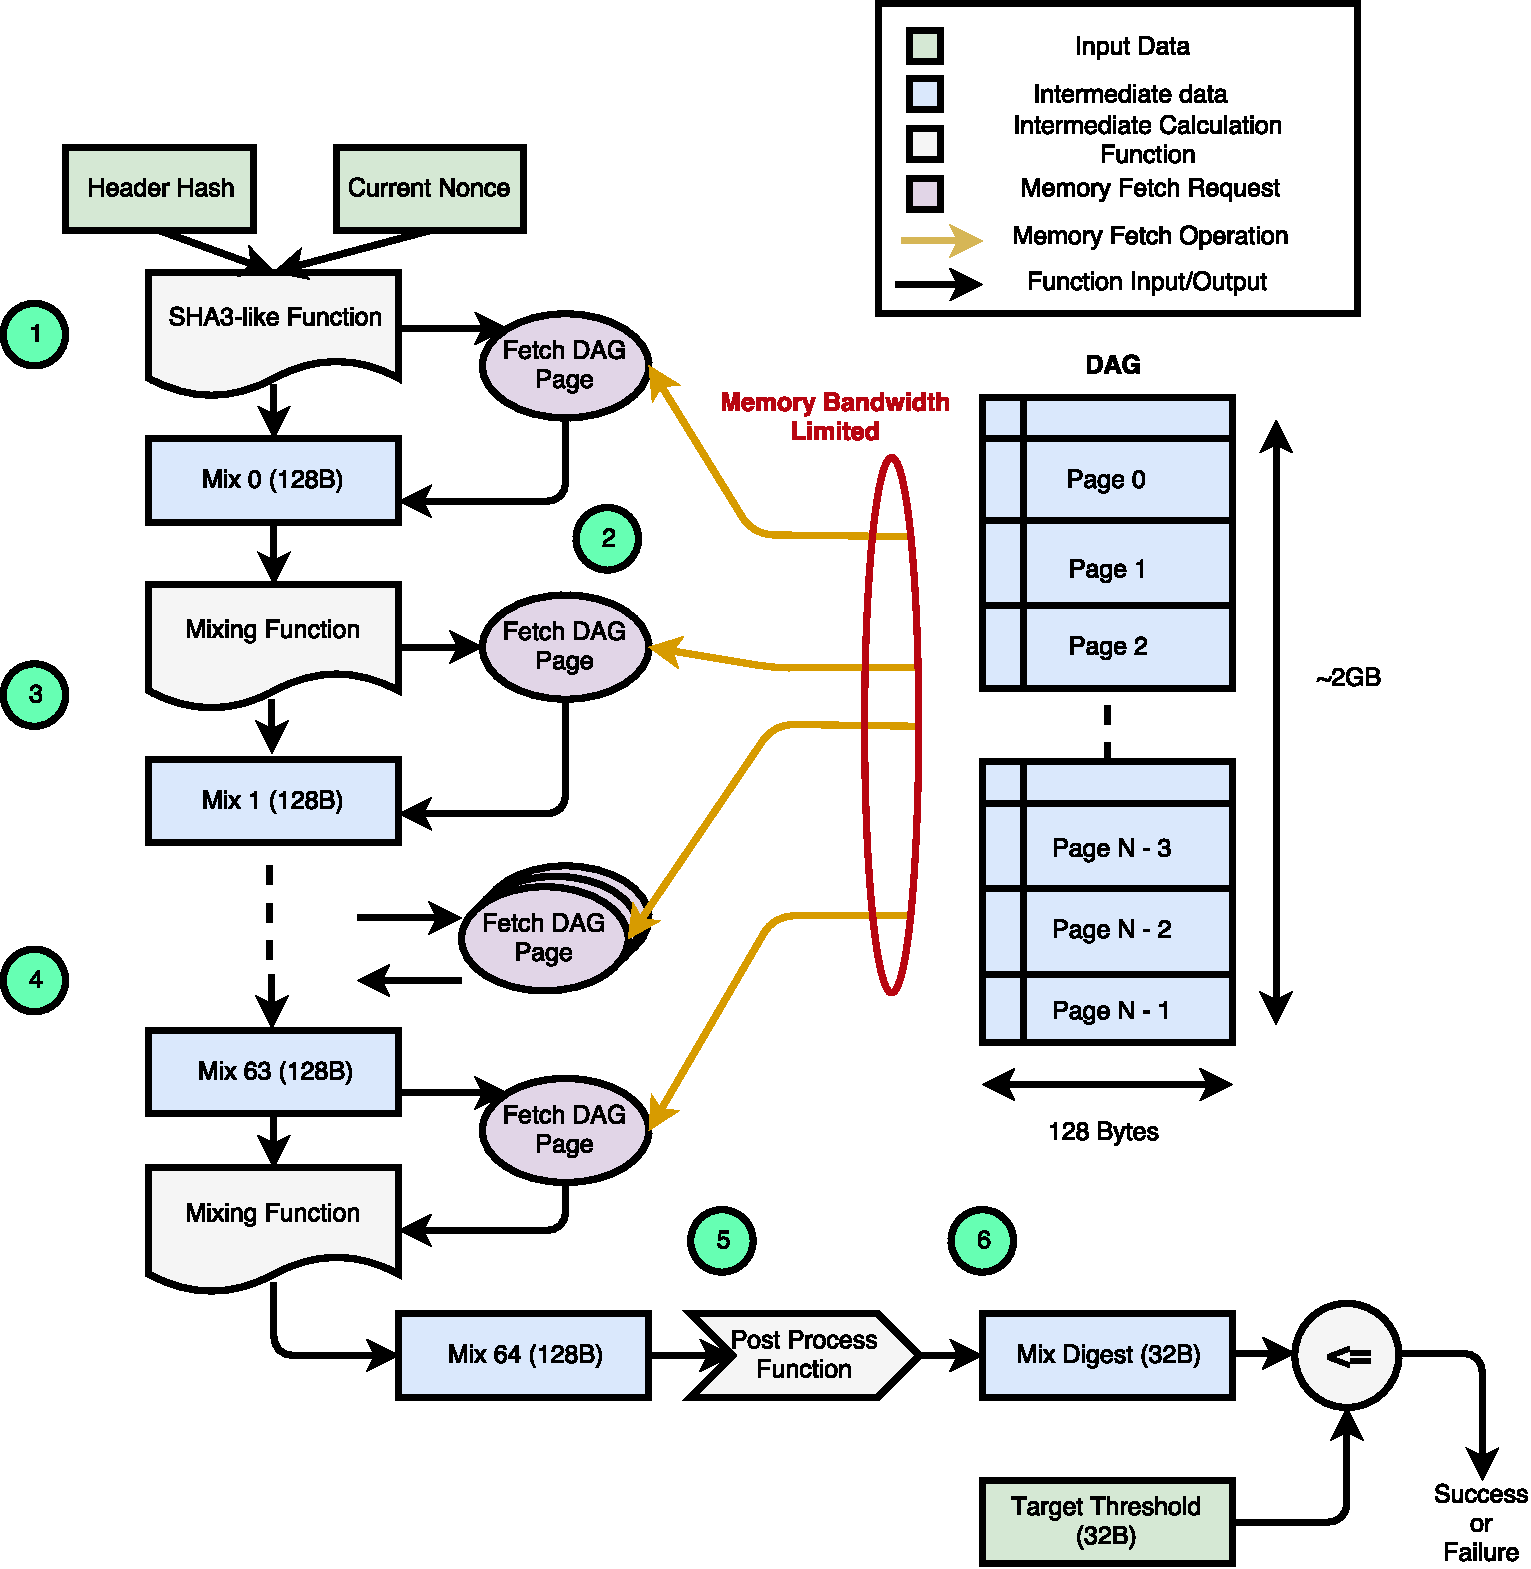
\includegraphics[width=300px,keepaspectratio]{Ethash.pdf}
\caption{\label{fig:ethash} Ethash}
\end{figure}

\subsection{Challenges}
\trishita{Too long of a sentence; need to reword}Given that we now know that the crux of having a good hashrate for Ethereum lies in having quick access to the DAG, one of the biggest challenges with mining it on a distributed ensemble of browsers would be to transfer and store this data structure within each worker browser. However, given that the DAG for an Ethereum network is at least 1GB (and growing) in size transferring it to the browser every time a client loads our web page would be impractical. Furthermore, even if we somehow manage to transfer the DAG to the client when the web page loads, the browser would still have to store it in memory, thereby using a sizeable amount of resources on the client machine. We attempt to address some of these concerns through our approach as discussed in the next section. 

\section{Our Approach}
We propose a lazy-evaluation based approach to alleviate the network and memory requirements for mining Ethereum in a distributed scenario on browsers. Specifically, as soon as each browser connects to the webserver, the server sends it the current header of the block being mined and the Cache. Once the browser receives the Cache, it allocates an array buffer to store the DAG slices that fall between indices 0 and $n$ that will be computed in the future. (Note that the $n$ is a variable parameter reflecting the length of the buffer with which we experiment in our analysis). Once the buffer is allocated, the browser can start iterating over nonces to compute hashes.  

Since, to begin with, the browser does not have any slices of the DAG, it must compute each slice on the fly using the Cache. However, for every such slice that the browser computes, it then stores it in the buffer (if it fits within the allocated bounds, otherwise it is simply discarded), for quicker access in the future. Hence, as time passes, the buffer starts filling up and so more and more slices are quickly accessed from the buffer rather than being computed from the ground-up, which makes hash computations faster with time. This has the effect that the longer the user remains on the web-page, the better the hashrate gets for that user. 

\subsection{Architecture}
% \begin{figure}[H]
% \centering
% \includegraphics[width=250px,keepaspectratio]{miningpool.png}
% \caption{\label{fig:miningpool} Distributed Ethereum Mining}
% \end{figure}

Our architecture was centered around two client-side Ethereum miners written in \verb|JavaScript| and \verb|WebAssembly|. The central node that co-ordinates all workers (browsers) was an improvised version of \verb|geth| ~\cite{geth}, a real world Ethereum miner written in \verb|Go|. \verb|Geth| typically runs as a standalone miner that mines on the machine it is running. We modified it so that instead of mining all by itself, it simply sends over the necessary data needed to mine (the hash of the Block Header and the Cache) to any client that connects to it on port \verb|9000|. After recieving the necessary data, the browser allocates a buffer for the DAG in order to store future slices. Note that the buffer for the DAG is implemented as an array of ints (with a DAG slice being 16 ints long), so as to make each lookup in the buffer $\theta(1)$. At this point, it can then begin to search for a solution. 

For our miner, we modeled our \verb|JavaScript| implementation based on the ~\verb|node.js| implementation of Ethash ~\cite{ethash}. To begin, the miner creates a random nonce and computes the hash (using the Cache and the buffered DAG) as discussed in the previous section. It will continue to perform this action on new nonces until one of two scenarios occur; it finds a nonce such that the computed hash is below the given threshold or the process has timed out. In the former case, the browser submits the result back to the node and then asks the node for a new block header and the Cache. Otherwise if it has timed out without finding a result, the browser simply polls the node for the current block header and Cache . This process will continue until the user moves away from the website or closes their browser. 
We must point out that this time out is necessary since we want the browser to work with the most recent block header and Cache. The block header can become stale if that particular block has already been mined, and the Cache can become stale if the Ethereum network transitions into a new Epoch (happens once every 30,000 blocks). 
We must point out that both our current implementations in \verb|JavaScript| and \verb|WebAssembly| require no external dependencies, and therefore can be directly embedded into any website. For a diagramatic view our our design, see Figures~\ref{fig:hybridArchitecture}.

\begin{figure}[h]
\centering
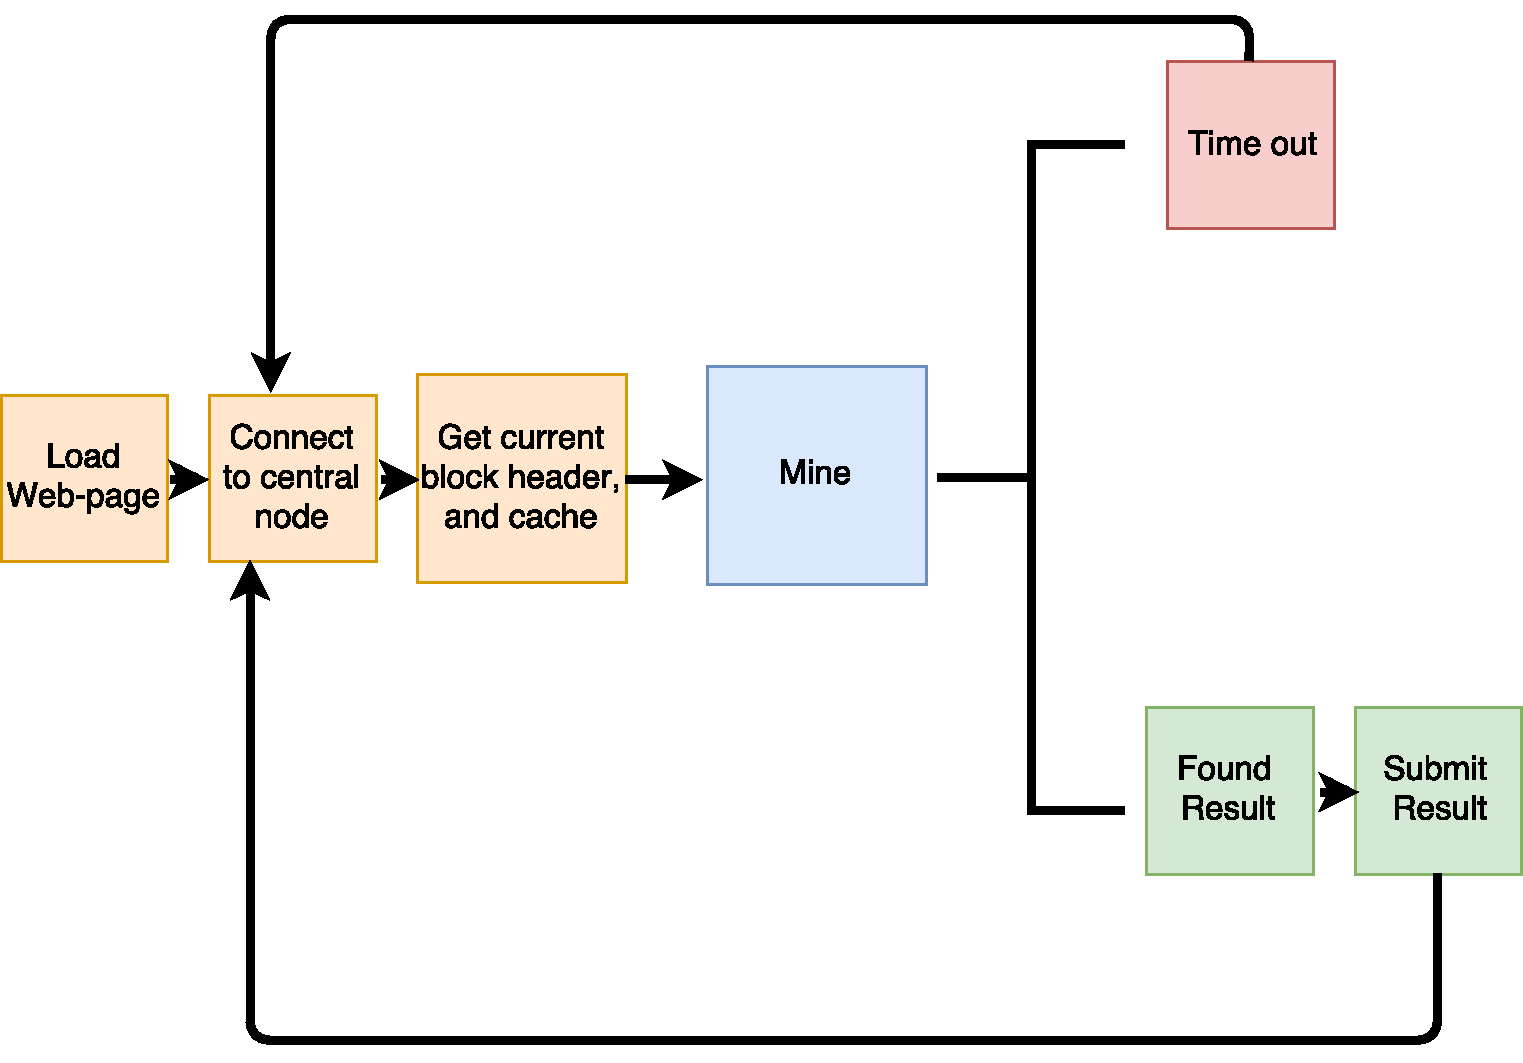
\includegraphics[width=230px,keepaspectratio]{Hybrid-Miner.pdf}
\caption{\label{fig:hybridArchitecture} Web Miner Architecture}
\end{figure}

\subsection{Theoretical Analysis}
With this lazy-evaluation based approach, we can calculate exactly how many hashes we would have to compute in order to fill up a buffer of a given size. This is important because once the buffer in the browser fills up, the hash rate that the browser gives is at its maximum, steady-state. In this section, we will mathematically demonstrate that filling a buffer the size of the DAG up should take at most 4.5 million hashes, while filling up 95\% of this buffer takes merely 800k hashes. This is a significant difference since in our experimental set-up, the browser takes X s to compute 4.5 million hashes, while only Y s to compute 800k hashes. The approach we take is similar to the Coupon Collector problem \cite{couponCollector}, and is discussed below. Note that for simplification, we assume that the DAG is randomly sampled in order to compute hashes. In reality, this is not entirely true and hence the results we obtain from this analysis are more conservative than what we see in practice. In fact, while we show here that filling up 95\% of a buffer as big as the DAG takes 800k hashes, whereas in reality it only takes half as many hashes~\ref{section:Results} \\

\makebox[\textwidth][l]{If we define}
\makebox[\textwidth][c]{Number of DAG slices = N}
\makebox[\textwidth][c]{Fraction of the DAG we want to buffer = $f_1$}
\makebox[\textwidth][c]{Number of DAG slices needed to compute a single hash = a}
\makebox[\textwidth][c]{Failure probability of finding a specific slice in the buffer (Buffer miss rate)= $\delta$}
% \makebox[\textwidth][c]{Failure probability of computing a hash just using slices in the buffer = $\omega$}
\makebox[\textwidth][c]{nth Harmonic Number = $H_n$}
% \makebox[\textwidth][c]{Euler-Mascheroni constant = $\gamma = 0.57721566...$}
% \makebox[\textwidth][c]{Expected number of hashes it takes to fill the buffer = E(H)}
% \begin{gather}\label{eq:slicevshash}
% 	(1-\delta)^a = 1-a\delta;\;\delta \to 0 %1-\omega
% \end{gather}
% \makebox[\textwidth][l]{When $\delta \to 0$, equation \ref{eq:slicevshash} can be re-written as}
% \begin{gather}
% 	1-a\delta = 1-\omega \\
%     \label{eq:deltaomega}
% 	a\delta = \omega
% \end{gather}
% \makebox[\textwidth][l]{Hence, the probability that a specific slice is present in the buffer}
% \begin{gather}
% 	1-\delta = 1-\frac{\omega}{a}
% \end{gather}
The number of slices $n$ needed to fill up a buffer of size $f_1$ for a given $\delta$ is given by:
\begin{gather}
	n = Nf_1(1-\delta) %= Nf_1(1-\frac{\omega}{a})
\end{gather}
This means that we are willing to allocate a buffer that is fraction $f_1$ of the entire DAG, but instead of filling up all $Nf_1$ slices, we are willing to forgo $Nf_1\delta$ slices. Using the Coupon Collector proof~\cite{couponCollector}, we know that the expected number of trials $E(t)$ of obtaining the $xth$ new slice after having buffered $x-1$ slices is:\\
\begin{gather}
	E(t_x) = \frac{Nf_1}{Nf_1-(x-1)}
\end{gather}
we see that the expected number of trials in order to obtain $n$ slices is given by
\begin{gather}
	E(t) = \sum_{x=1}^{n}E(t_x) = Nf_1\sum_{x=1}^{n}\frac{1}{Nf_1-x+1} = Nf_1\sum_{x=1}^{Nf_1(1-\delta)}\frac{1}{Nf_1-x+1}
\end{gather}
Splitting this into two summations,
\begin{gather}
	E(t) = Nf_1[\sum_{x=1}^{Nf_1}\frac{1}{Nf_1-x+1} - \sum_{x=Nf_1(1-\delta)+1}^{Nf_1}\frac{1}{Nf_1-x+1}] \\
    E(t) = Nf_1[H_{Nf_1} -H_{Nf_1\delta}] \\
    \label{eq:expectedHashes}
	E(H) = \frac{Nf_1}{a}[H_{Nf_1} -H_{Nf_1\delta}]
\end{gather}
Now, using equation ~\ref{eq:expectedHashes}, bounds on Harmonic Numbers ~\cite{harmonicNumber}, and setting $N = 16777186$, $f_1 = 1$, $a = 64$ and $\delta = 0.95$, we get $E(H) = 785312$ hashes.
Hence, we see that even computing merely 800k hashes fills a DAG buffer as large as the entire DAG by more than 95\%, as opposed to calculating 4.5 million to fill the buffer entirely. (Note that this number should be smaller for smaller buffer sizes; so this is again a rough upper bound). This suggests that the fuller the buffer is, the marginal cost of computing more hashes outweighs the rate at which the buffer is filled up. In fact, as we will see in the results, filling up 95\% of a buffer as large as the DAG already starts giving us good hash rates for a browser (10kH/s). 
This means that reaching a reasonably steady state is not as hard as it seems at face value, making this approach viable for web setting where users might not stay on websites for long. Given this result, we compute 800k hashes for all our experiments, as discussed in the next section.



%%%%%%%%%%%%%%%%%%%%%%%%%%%%%%%%%%%%%%
% \begin{theorem}[Expectation of Number of Hashes]
% \label{expectedHashes}\\
% \makebox[\textwidth][l]{If we define}
% \makebox[\textwidth][c]{Number of DAG slices = n}
% \makebox[\textwidth][c]{Size of buffer as a fraction of the total DAG = $f_1$; $f_1$=[0,1]}
% \makebox[\textwidth][c]{Expected number of hashes it takes to fill the buffer = E(H)}
% \makebox[\textwidth][c]{nth Harmonic Number = $H_n$}
% \makebox[\textwidth][c]{Euler-Mascheroni constant = $\gamma = 0.57721566...$}
% \makebox[\textwidth][c]{Probability of obtaining a new slice after having buffered x slices = $P_x = \frac{nf_1-x}{n}$}
% \makebox[\textwidth][c]{Expected number of trials $t_x$ to get a new slice after having seen} 
% \makebox[\textwidth][c]{$x$ out of $nf_1$ slices = 
% $E(t_x) = \frac{1}{P_x} = \frac{n}{nf_1-x}$}
% \makebox[\textwidth][c]{Expected number of trials it would take to see all $x$ slices = $E(t)$}
% % ~\trishita{add reference to results}
% From the Coupon Collector Problem~\cite{couponCollector}, it follows that:
% \begin{gather}
% E(t) = \sum_{x=0}^{nf_1-1}E(t_x) = \sum_{x=0}^{nf_1-1}\frac{1}{P_x} = n\sum_{x=0}^{nf_1-1}\frac{1}{nf_1-x} = nH_{nf_1}
% \end{gather}

% It then follows from bounds on the nth Harmonic Number~\cite{harmonicNumber} that the expected number of hashes $E(H)$ it takes to fill up a buffer of fraction $f_1$ of a DAG with $n$ slices is bounded by:
% \begin{gather}
% \frac{n}{64}[\ln{nf_1} + \frac{1}{2nf_1} + \gamma - \frac{1}{12({nf_1})^2+2\frac{7-12\gamma}{2\gamma - 1}}] <= E(H) \\ E(H)< \frac{n}{64}[\ln{nf_1} + \frac{1}{2nf_1} + \gamma - \frac{1}{12({nf_1})^2+\frac{6}{5}}] 
% \end{gather}

% this was the proof for the expression above
% % \end{theorem}
% % \begin{proof}
% Let us assume we have a buffer for our DAG that is $f_1$ as large as the entire DAG -- i.e., the buffer can only store dag slices with indices $i$ such that $i \in [0,nf_1]$. Hence, each time we calculate a DAG slice from the Cache, we may or may not buffer it depending on whether it falls within the index rage. Now, let us assume that  we have buffered $x$ slices so far, the probability of obtaining a new slice is given by:
% \begin{gather}
% 	P_x = \frac{nf_1-x}{n}
% \end{gather}
% The event of obtaining a new slice after having already collected $x$ out of the $nf_1$ slices that can be buffered can be modeled as a geometric distribution. Hence, the expected number of trials $t_x$ it takes to get a new  slice after having seen $x$ out of the $nf_1$ slices is:
% \begin{gather}
% 	E(t_x) = \frac{1}{P_x} = \frac{n}{nf_1-x}
% \end{gather}
% By linearity of expectation, the total number of trials it would take to see all $x$ slices is:
% \begin{gather}
% 	E(t) = \sum_{x=0}^{nf_1-1}E(t_x) = \sum_{x=0}^{nf_1-1}P_x = \sum_{x=0}^{nf_1-1}\frac{n}{nf_1-x} = n\sum_{x=0}^{nf_1-1}\frac{1}{nf_1-x}
% \end{gather}
% Since the summation represents the harmonic series, the expected value can be approximated as follows:
% \begin{gather}
% 	E(t) = n\log{nf_1}
% \end{gather}
% Equation ~\ref{eq:7} is in terms of the number of individual accesses of the DAG. In order to get the expected number of Hashes (as opposed to the expected number of individual DAG slice accesses), we need to divide by 64 since each hash involves 64 accesses of the DAG. Hence: 
% \begin{gather}
% 	E(H) = \frac{E(t)}{64} = \frac{n\log{nf_1}}{64}
% \end{gather}
% \end{proof}


% The factor of 64 comes from the fact that calculating each hash requires sampling the DAG 64 times. Given this, let us do a simple calculation for one extreme case, where we allocate a buffer as large as the entire DAG on the browser (in order to get an upper bound on the number of hashes it would take to fill this buffer up). Here $f_1 = 1$ and $n = 16777186$ (for our private test network), which, using ~\ref{eq:6}, gives us $4512210 < E(H) <= 4512210$ hashes. Hence, it takes around 4.5 million hashes to fill up a buffer as large as the entire DAG. If $f_1 < 1$, the number of hashes should be less than 4.5 million, thus making it a very loose upper bound on the number of hashes needed to fill up a DAG buffer (and thereby reaching a steady-state hash rate). 

% In practice, however, we do not need to wait till the buffer is \emph{completely} full till we see good hash rates. We will demonstrate how we can get away with a much smaller number of hashes to fill up \emph{almost all} of the buffer, thereby reaching very good hash rates relatively quickly.


% lower bound (python exp): (n/64.0)*(log(n) + 1.0/(2*n) + g - 1.0/(12*(n**2) + (2*(7-12*g)/(2*g-1))))
% upper bound (python exp): (n/64.0)*(log(n) + 1.0/(2*n) + g - 1.0/(12*(n**2) + 6.0/5))

% Now let us say that we do not want to wait for the entire buffer to fill up -- how many hashes would we have to compute until a reasonable fraction of the buffer is full? For this, we have the following corollary:
% \begin{corollary}
% \label{earlyTermination}
% \makebox[\textwidth][l]{If we further define,}
% \makebox[\textwidth][c]{Fraction of DAG buffer to be filled = $f_2$; $f_2$ $\in$ [0,1]}
% \makebox[\textwidth][c]{$x  = E(H) - \frac{n}{64}\ln{\frac{nf_1}{nf_1 - nf_2f_1 - 1}} - \frac{1}{128f_1} + \frac{n}{768({nf_1})^2+128\frac{7-12\gamma}{2\gamma - 1}}$}
% \makebox[\textwidth][l]{Then,}
%     \begin{gather}
%    \frac{n}{768({nf_1 - nf_2f_1 - 1})^2+128\frac{7-12\gamma}{2\gamma - 1}} - \frac{1}{768({nf_1})^2+128\frac{7-12\gamma}{2\gamma - 1}} < x \\
%    x <= \frac{n}{768({nf_1-nf_2f_1-1})^2+\frac{6}{5}} - \frac{n}{12({nf_1})^128+\frac{6}{5}} 
% 	\end{gather}
% % \end{corollary}
% % \begin{proof}
% Then, for a buffer with space for $f_1$ slices, the number of slices we want to fill it with in order for a fraction $f_2$ of it to be full would be: \\
% \makebox[\textwidth][c]{Number of slices to fill DAG buffer with = $nf_2f_1$}
% This would modify equation \ref{eq:6} for the expected number of trials as follows:
% \begin{gather}
%     E(t) = \sum_{x=0}^{nf_2f_1}\frac{1}{P_x} = \sum_{x=0}^{nf_2f_1}\frac{n}{nf_1-x} = n\sum_{x=0}^{nf_2f_1}\frac{1}{nf_1-x}
% \end{gather}
% This is essentially an early termination of the summation in equation ~\ref{eq:6}, and can be expressed as follows:
% \begin{gather}
%     E(t) = n\sum_{x=0}^{nf_2f_1}\frac{1}{nf_1-x} = n(\sum_{x=0}^{nf_1-1}\frac{1}{nf_1-x} - \sum_{x=nf_2f_1+1}^{nf_1-1}\frac{1}{nf_1-x}) \\
%     E(t) = n[H_{nf_1} - H_{nf_1 - nf_2f_1 - 1}]\\
% \end{gather}
% Again, using the bounds on the nth Harmonic Number~\cite{harmonicNumber}, substituting $\frac{E(t)}{64} = E(H)$ and $x$, and simplifying, we get the following: \\
% \makebox[\textwidth][l]{Let}
% \begin{gather}
% 	n[
%     \ln{\frac{nf_1}{nf_1 - nf_2f_1 - 1}} + \frac{1}{2nf_1} - \frac{1}{12({nf_1})^2+2\frac{7-12\gamma}{2\gamma - 1}} \\ - \frac{1}{2(nf_1 - nf_2f_1 - 1)} + \frac{1}{12({nf_1 - nf_2f_1 - 1})^2+2\frac{7-12\gamma}{2\gamma - 1}}] < E(t) \\
%     E(t) <= n(\ln{\frac{nf_1}{nf_1 - nf_2f_1 - 1}} + \frac{1}{2nf_1} - \frac{1}{12({nf_1})^2+\frac{6}{5}} \\
%     - \frac{1}{2(nf_1-nf_2f_1-1)} + \frac{1}{12({nf_1-nf_2f_1-1})^2+\frac{6}{5}}) \\
%     x  = E(H) - \frac{n}{64}\ln{\frac{nf_1}{nf_1 - nf_2f_1 - 1}} - \frac{1}{128f_1} + \frac{n}{768({nf_1})^2+128\frac{7-12\gamma}{2\gamma - 1}} \\
%    \frac{n}{768({nf_1 - nf_2f_1 - 1})^2+128\frac{7-12\gamma}{2\gamma - 1}} - \frac{1}{768({nf_1})^2+128\frac{7-12\gamma}{2\gamma - 1}} < x \\
%    x <= \frac{n}{768({nf_1-nf_2f_1-1})^2+\frac{6}{5}} - \frac{n}{12({nf_1})^128+\frac{6}{5}} 
% \end{gather}    
%     \ln{()}) \\
%     E(t) = n\log{\frac{1}{1-f_2-\frac{1}{nf_1}}}

% Again, we divide by 64 to obtain the expected number of hash computations:
% \begin{gather}
%     E(H) = \frac{n}{64}\log{\frac{1}{1-f_2-\frac{1}{nf_1}}}
% \end{gather}
% \end{proof}
%%%%%%%%%%%%%%%%%%%%%%%%%%%%%%%%%%%%%%%%%%%%%%%%%%

% Interestingly, since for realistic cases $n >> f_1$, $\frac{1}{nf_1} \to 0$, and so 
% \begin{gather}
% E(H) \approx \frac{n}{64}\log{\frac{1}{1-f_2}}
% \end{gather}
% Figure X shows a graph of how $E(H)$ varies as a function of the fraction of the buffer that we want to be full, $f$ if we set $n = 16777186$ (the total number of DAG slices on the experimental private test network). 

% Beyond that, the marginal cost of computing more hashes outweighs the rate at which the DAG is filled up. Hence, as we will see in the next section, for our experiments, we compute 800,000 hashes.

\section{Results}
\subsection{Experimental set up}
Our experimental set up consisted of a machine with an Intel i7-7700HQ processor with 8 cores and 16GB ram. These results were obtained from a private Ethereum test network at Epoch 0. The DAG size was 16777186 slices (1.074GB). The cache size was 1.677MB. We ran the implementations in ~\verb|JavaScript| and ~\verb|WebAssembly| in the browser, and a native miner written in ~\verb|C++| that employs the same approach outside of the browser for control results. Each miner was run till 800,000 hashes were computed and the hash rate and buffer hit rate were sampled every 10,000 hashes. (Note that both the hash rate and buffer hit rate sampled at a particular time reflected the values over the 10,000 most recent hashes).

% \subsection{Baseline results}
% For our control results, we ran \verb|Geth|~\cite{geth}, a native miner written in \verb|Go| that stores the entire DAG in memory from the start (as opposed to using this lazy evaluation approach), and obtained an average hashrate of X H/s. 

% We also ran our lazy-evaluation based miner written in C++ outside of the browser, and obtained the following results. 
% Figure X below shows a heat-map of how the hash rate varies as a function of both the size of the buffer allocated to store the DAG (as a percentage of the size of the entire DAG) and the number of hashes computed in the browser. Figures X then shows a heat-map of how the DAG buffer hit-rate varies as a function of both the size of the buffer allocated to store the DAG and the number of hashes computed in the browser. 

% . Since the hashrate determines how fast a mining rig can verify a nonce, it was necessary to ensure that our results were not skewed due to the differences in computing power between computers. Using this machine, we recorded the hashrates for CPU performance and GPU performance on our private Ethereum testnet. 
% Additionally, we also recorded the hashrates for CPU mining in a Kali Linux VM. As we can see in the figure below, the GPU clearly outperforms the CPUs resulting in an average hashrate of 5.72MH/s. As for the CPUs, both miners performed about the same, both hovering around a respectable 210kH/s.
% \begin{figure}[H]
% \centering
% \includegraphics[width=250px,keepaspectratio]{GPU.png}
% \caption{\label{fig:gpu} GPU vs CPU Hashrates}
% \end{figure}

% \begin{figure}[H]
% \centering
% \includegraphics[width=250px,keepaspectratio]{CPU.png}
% \caption{\label{fig:cpu} VM CPU vs CPU Hashrates}
% \end{figure}

\subsection{Implementation Results}
Figures~\ref{fig:NativeMinerHM},~\ref{fig:WebAsmMinerHM} and ~\ref{fig:JSMinerHM} below shows a heat-map of how the hash rate varies for each of the three implementations as a function of both the size of the buffer allocated to store the DAG (as a percentage of the size of the entire DAG) and the number of hashes computed in the browser. 
% \trishita{To Do: chanege to log scale, fix size }

\begin{figure}[h]
\centering
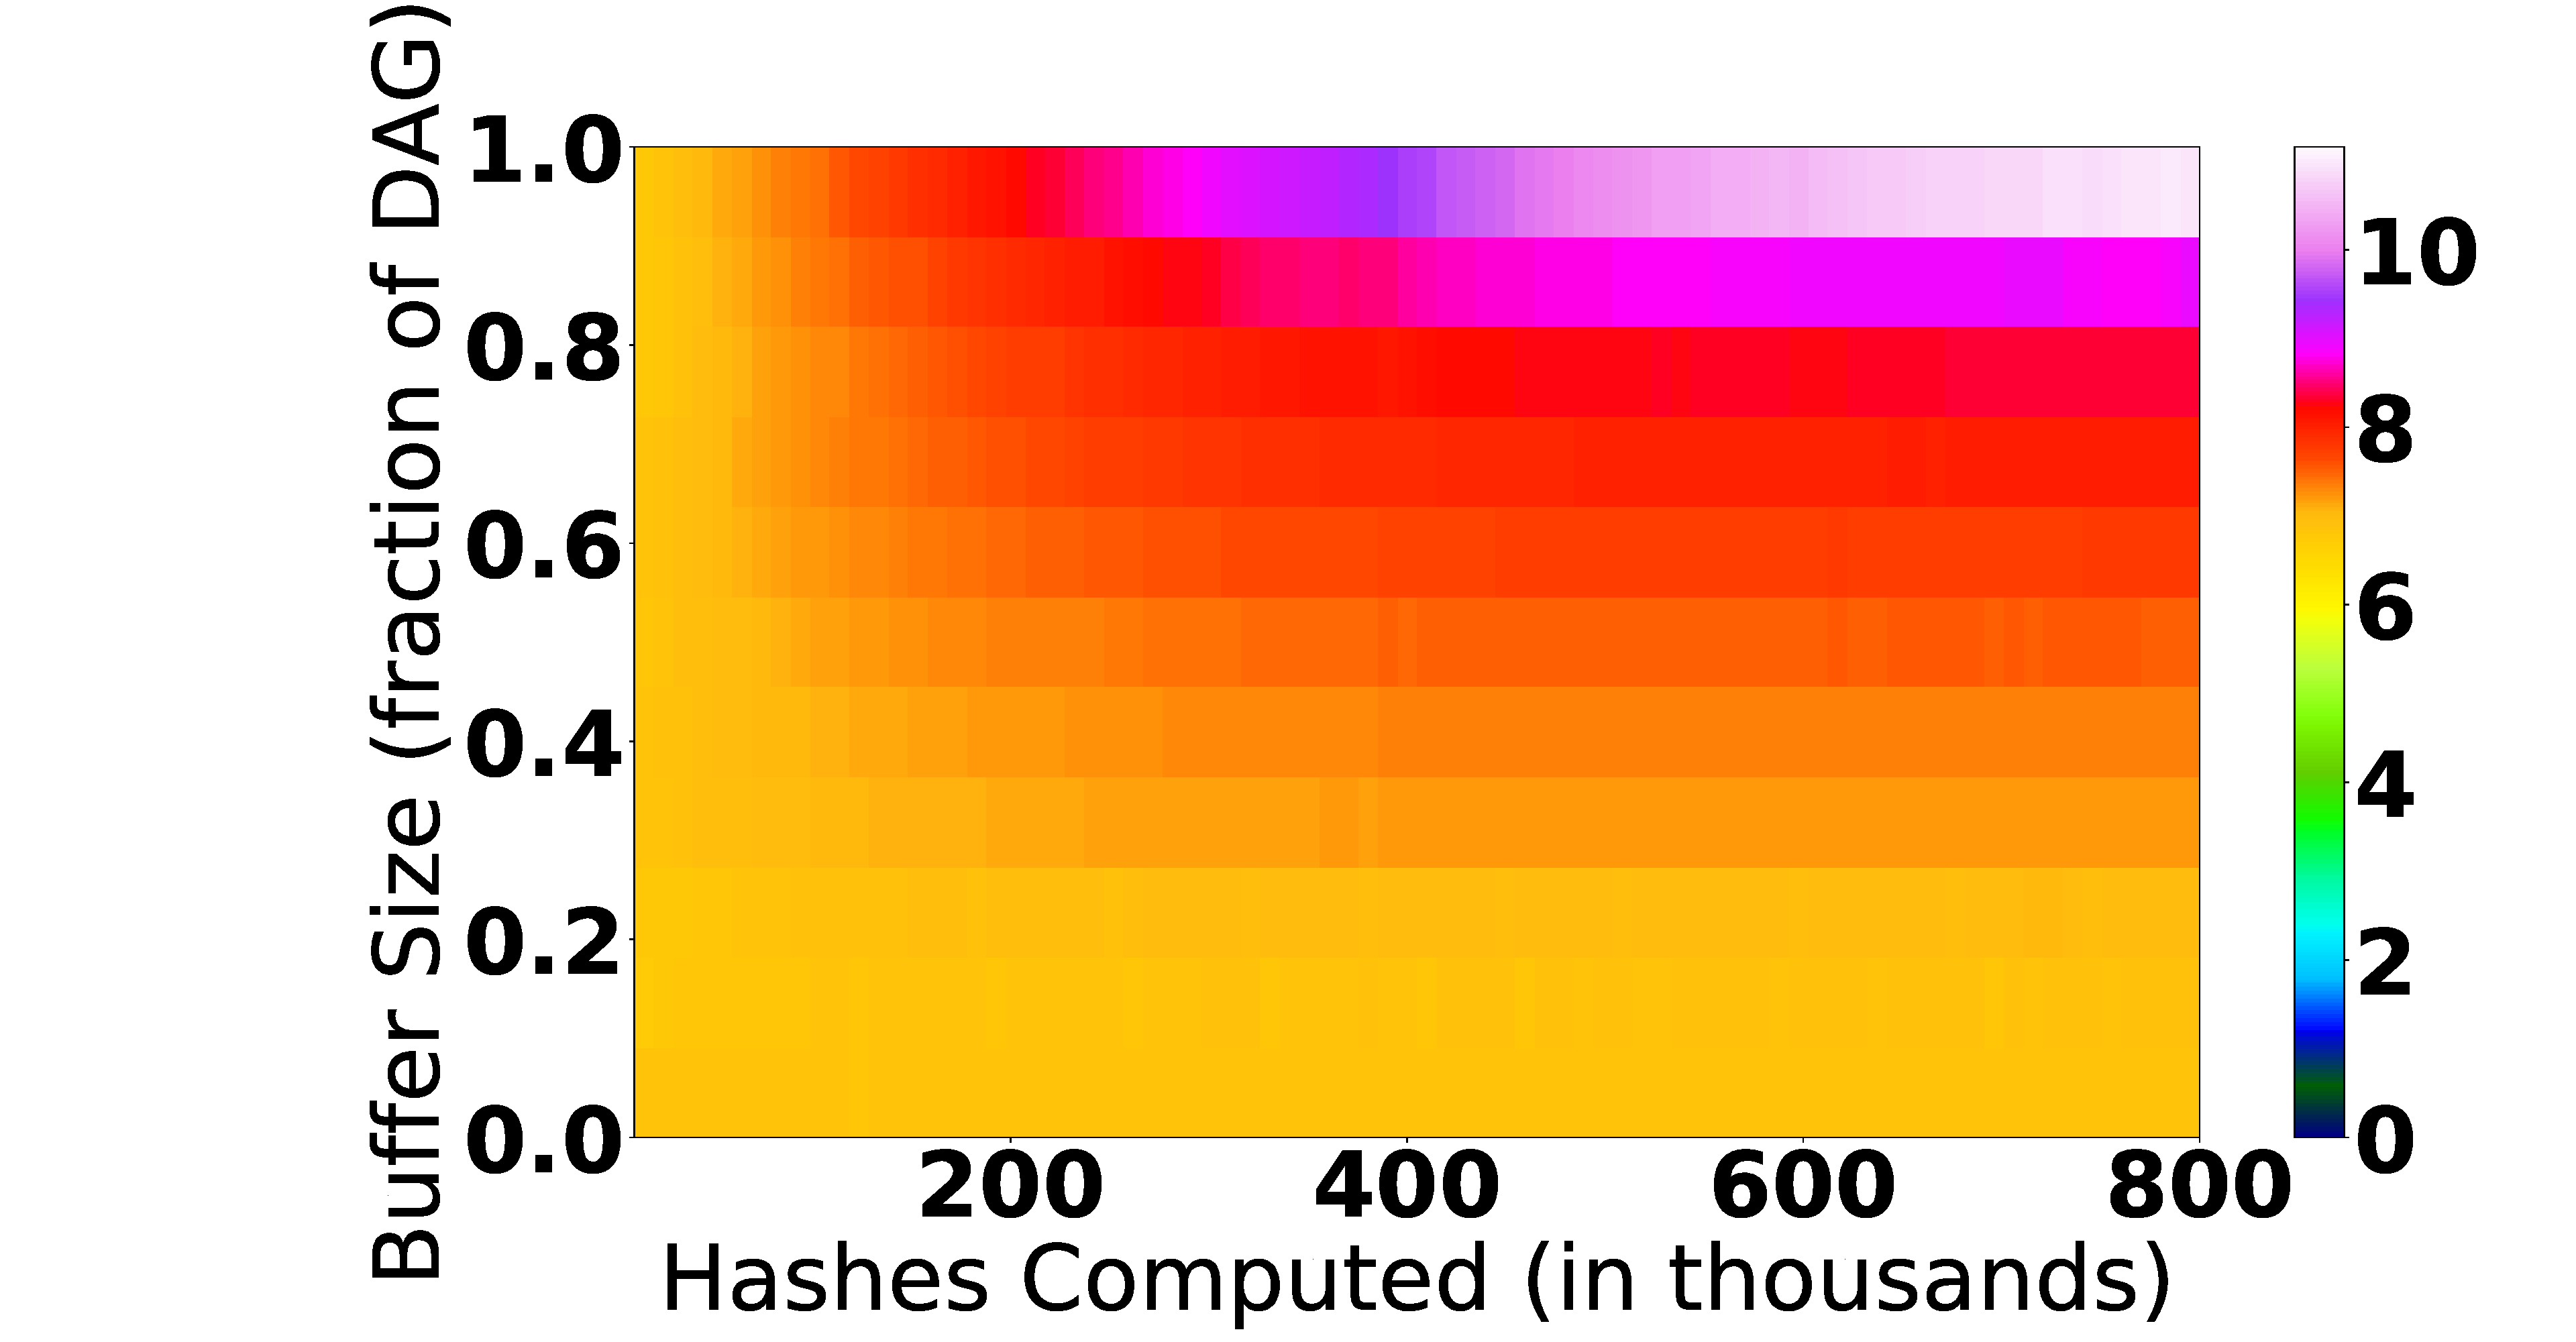
\includegraphics[width=250px,keepaspectratio]{Native_C++_Miner_Hash_Rate_HM.pdf}
\caption{\label{fig:NativeMinerHM} Native Miner: $\log{Hash Rate}$}
\end{figure}

\begin{figure}[h]
\centering
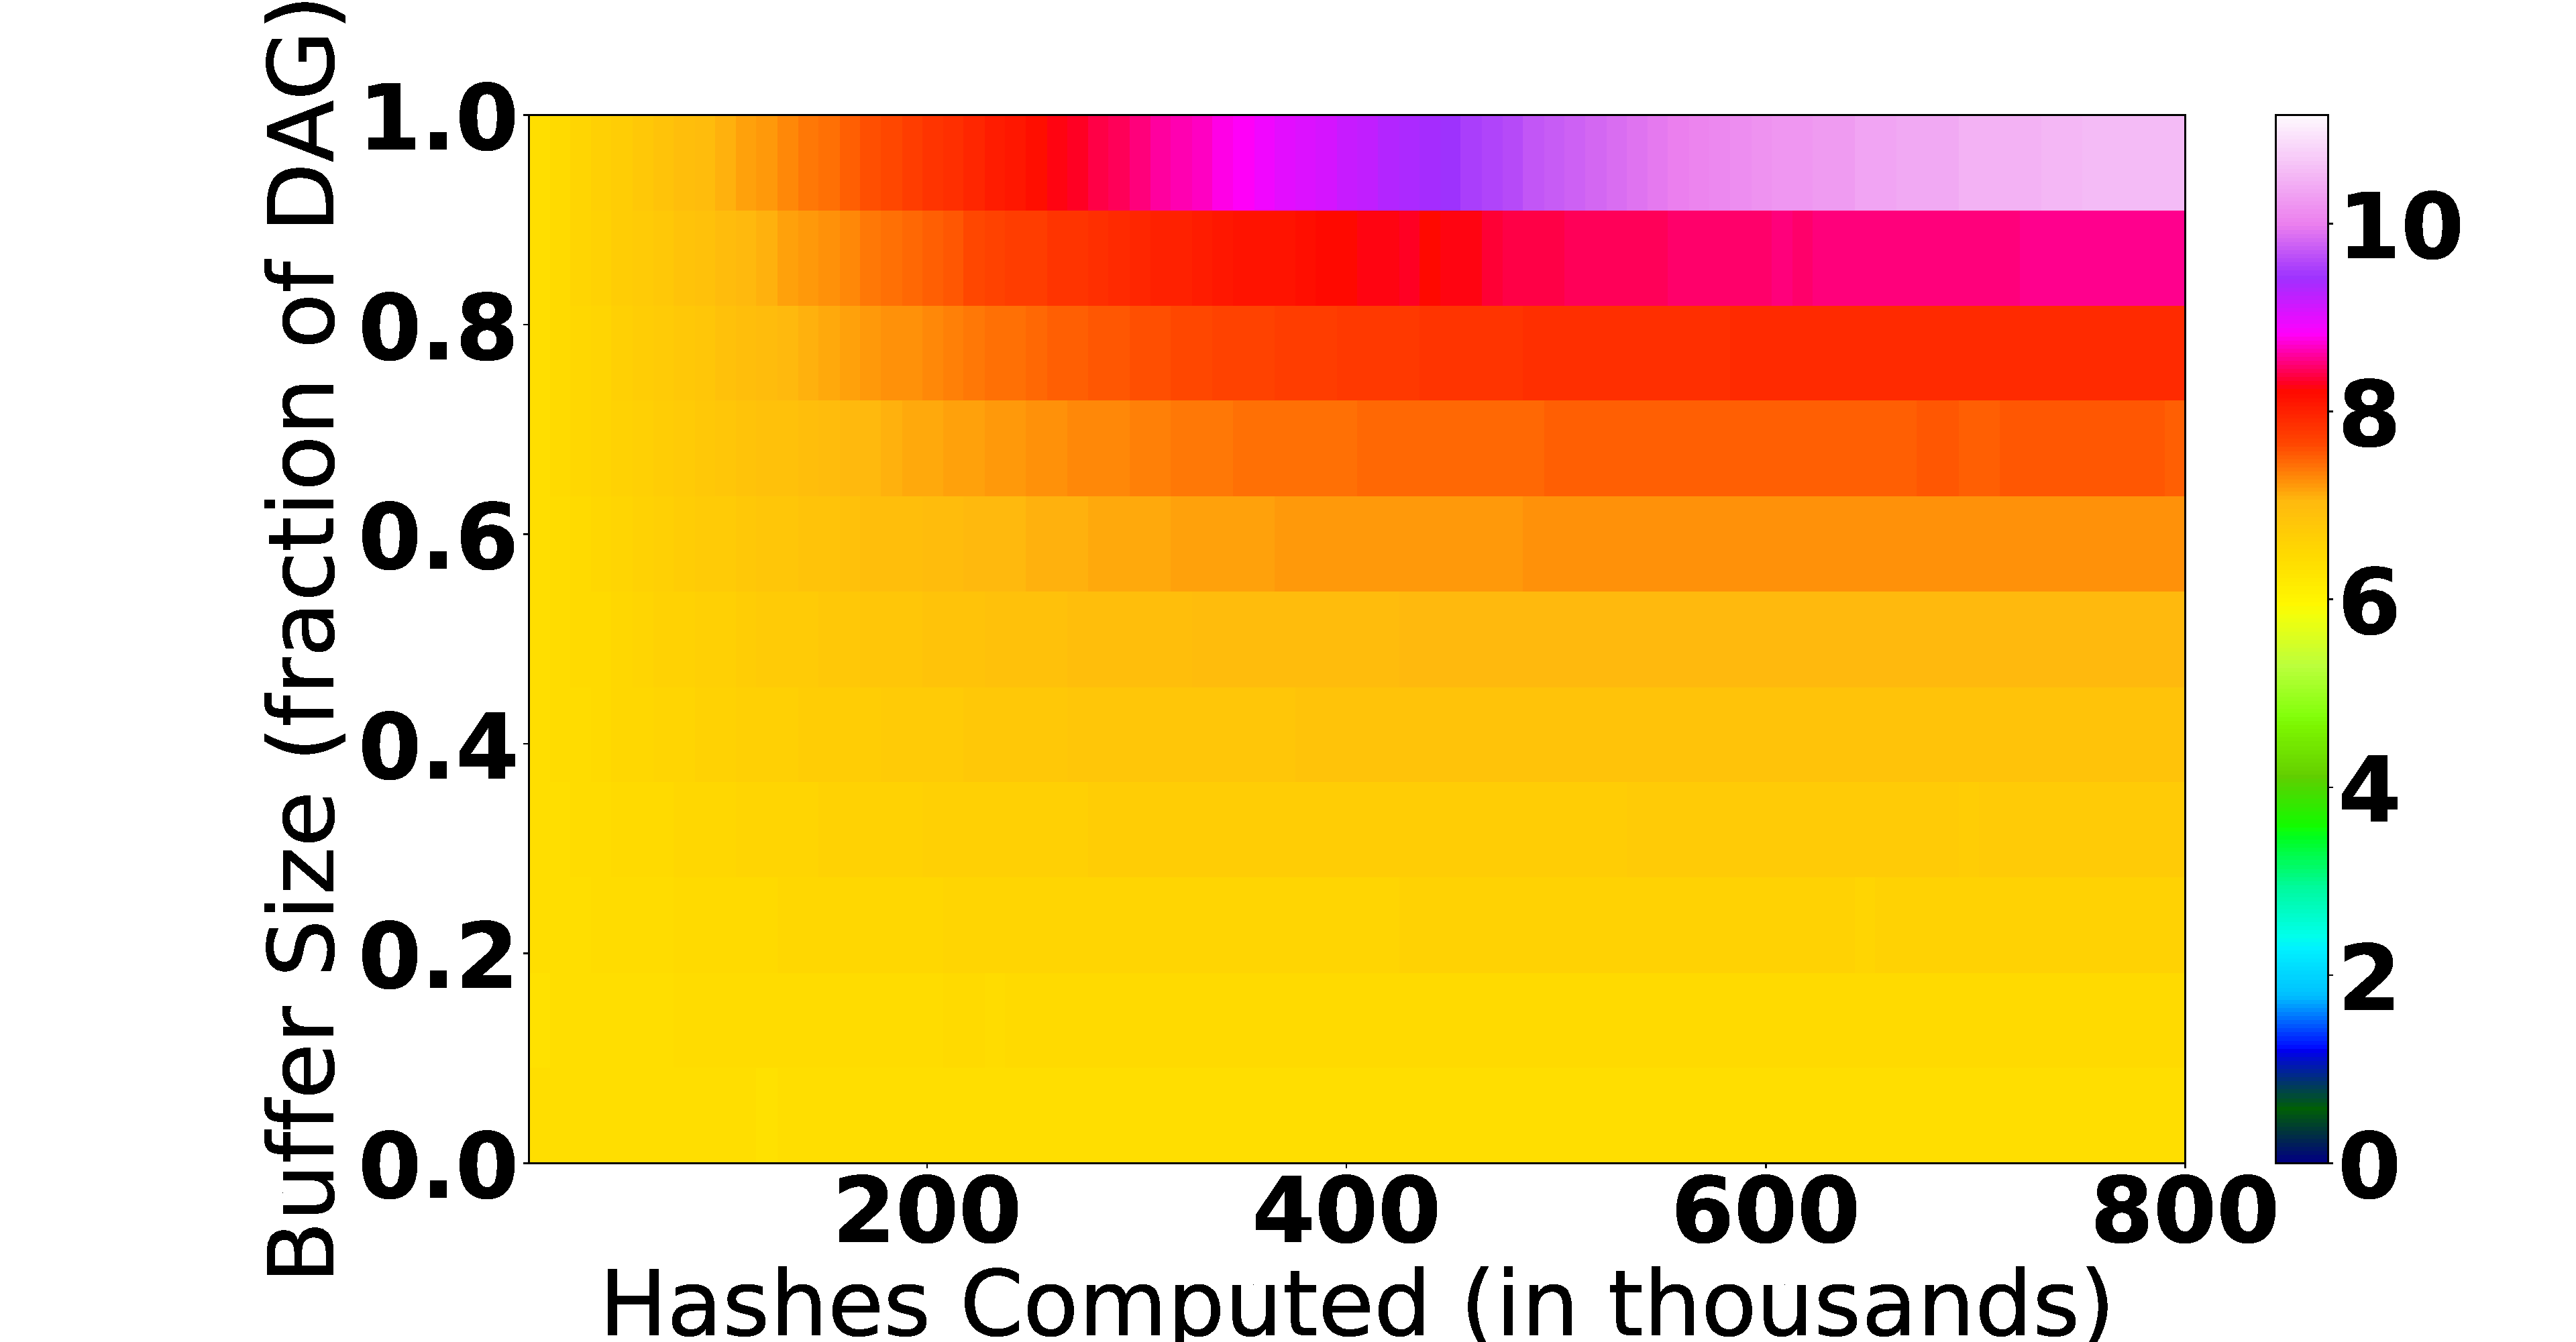
\includegraphics[width=250px,keepaspectratio]{WebAssembly_Miner_Hash_Rate_HM.pdf}
\caption{\label{fig:WebAsmMinerHM} WebAssembly Miner: $\log{Hash Rate}$}
\end{figure}

\begin{figure}[h]
\centering
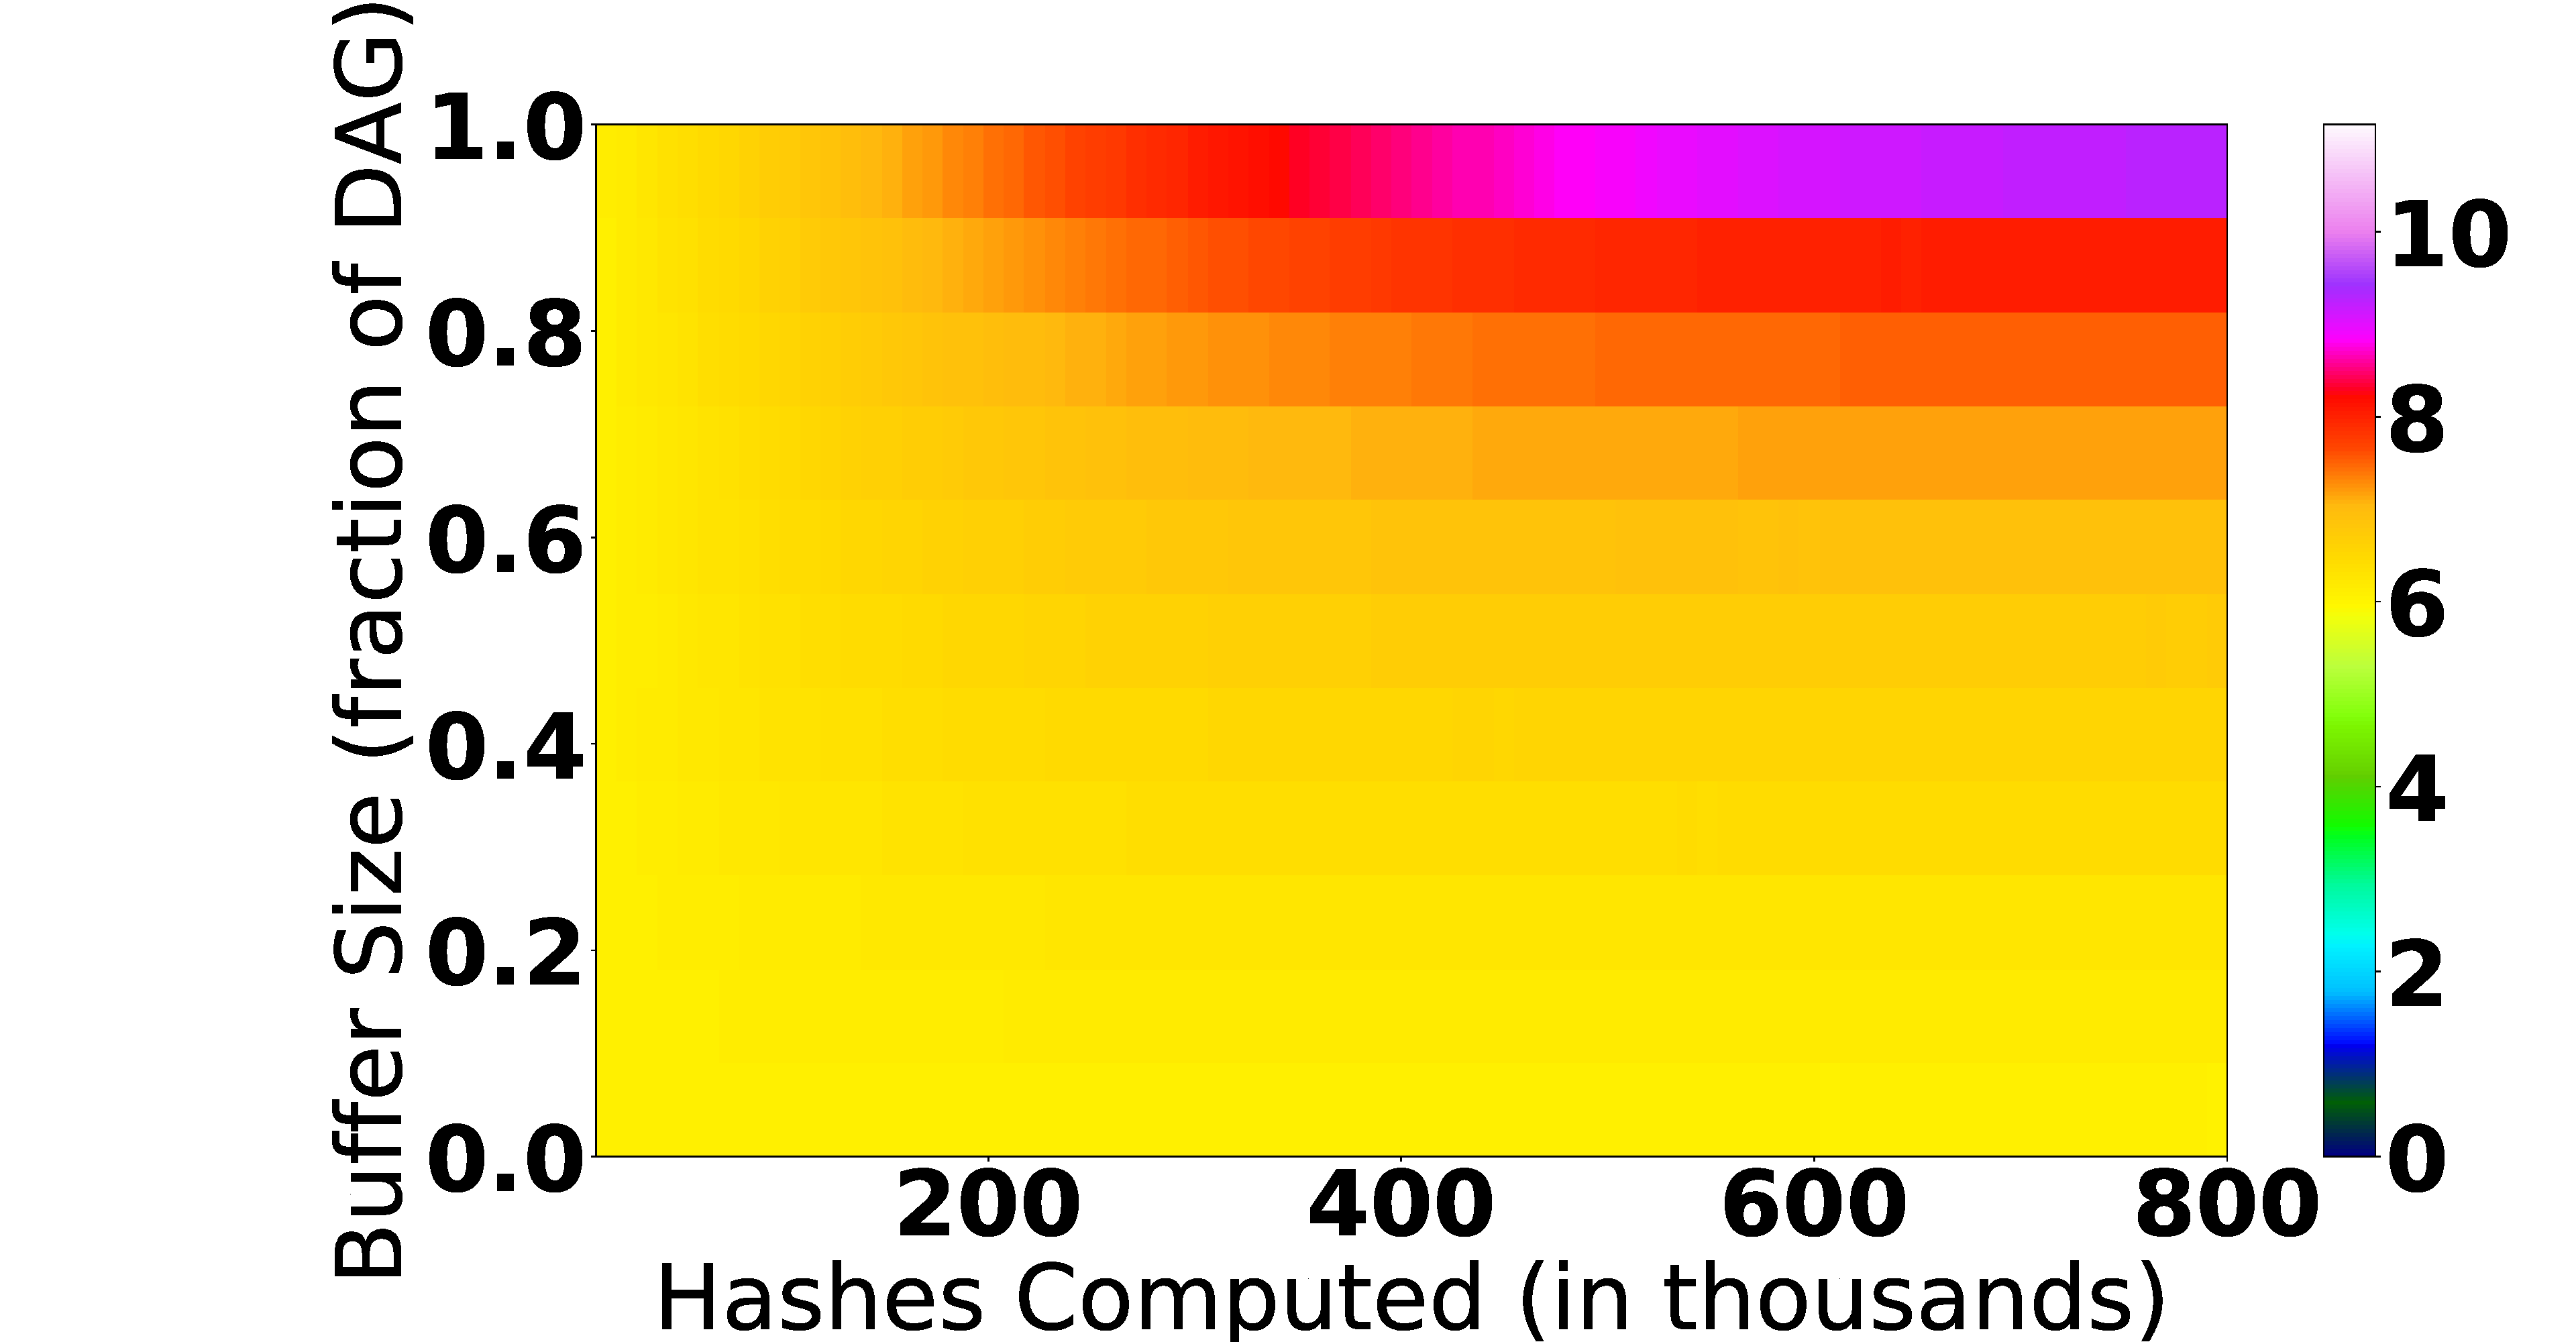
\includegraphics[width=250px,keepaspectratio]{JavaScript_Miner_Hash_Rate_HM.pdf}
\caption{\label{fig:JSMinerHM} JavaScript Miner: $\log{Hash Rate}$}
\end{figure}

% \begin{figure}[!htb]
% \minipage{\textwidth}
%   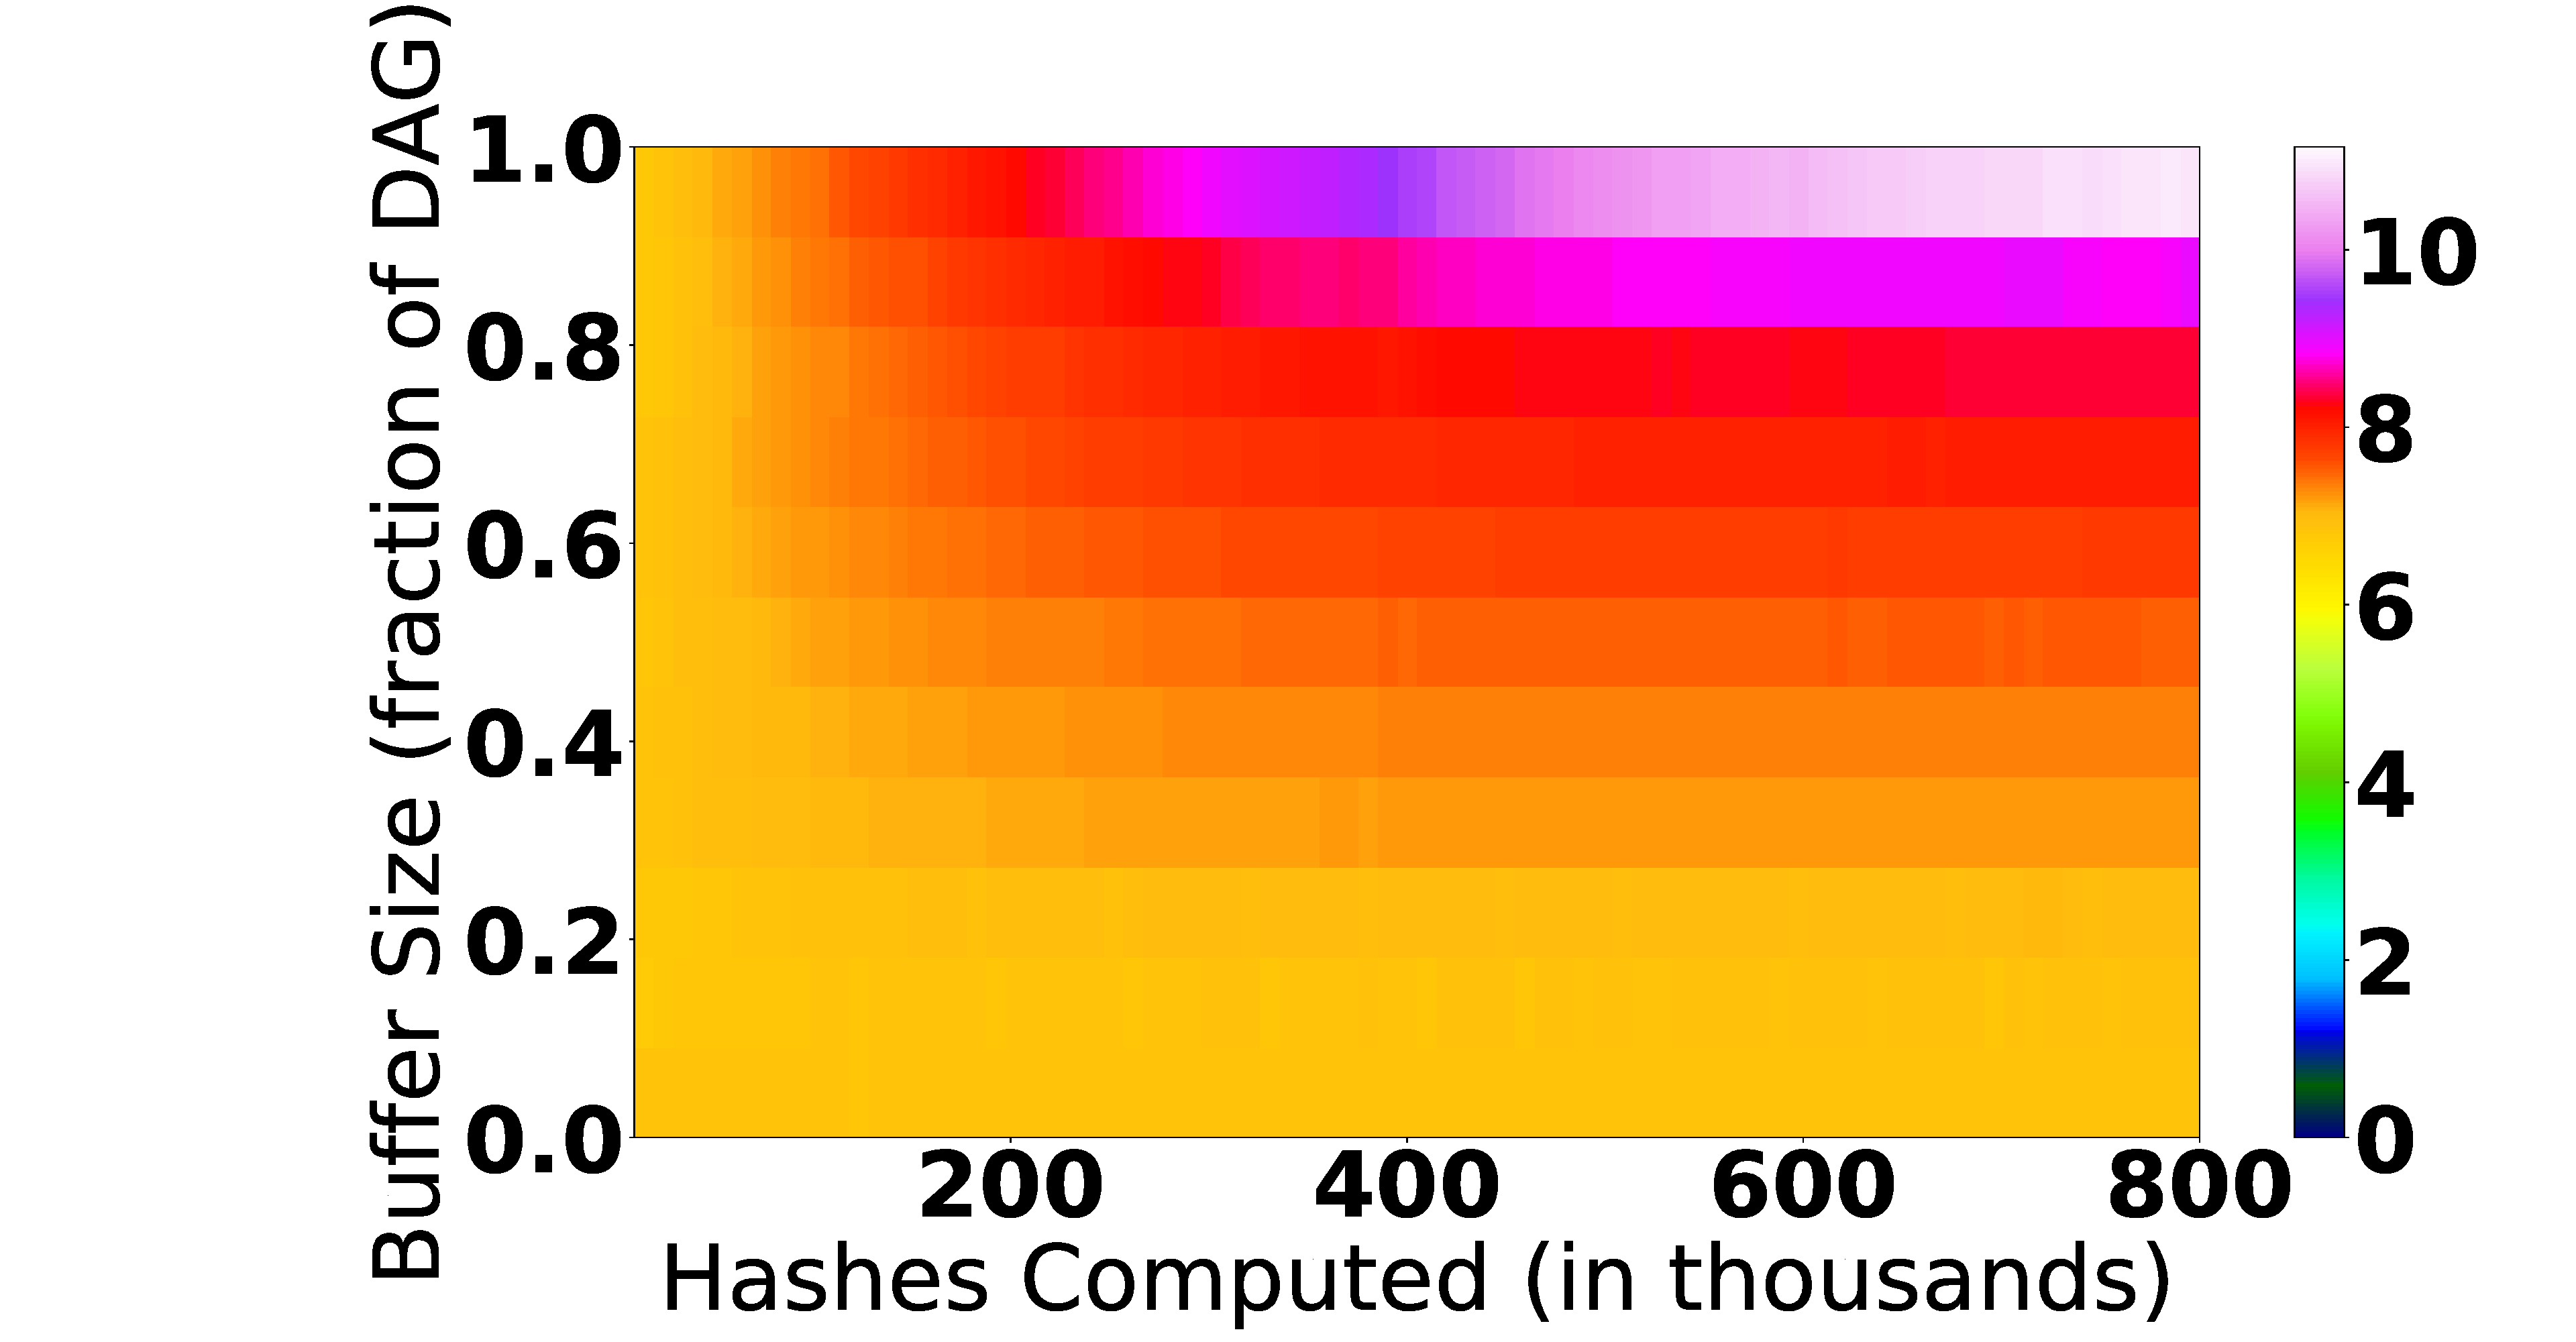
\includegraphics[width=\linewidth]{Native_C++_Miner_Hash_Rate_HM.pdf}
% \endminipage\hfill
% \minipage{\textwidth}
%   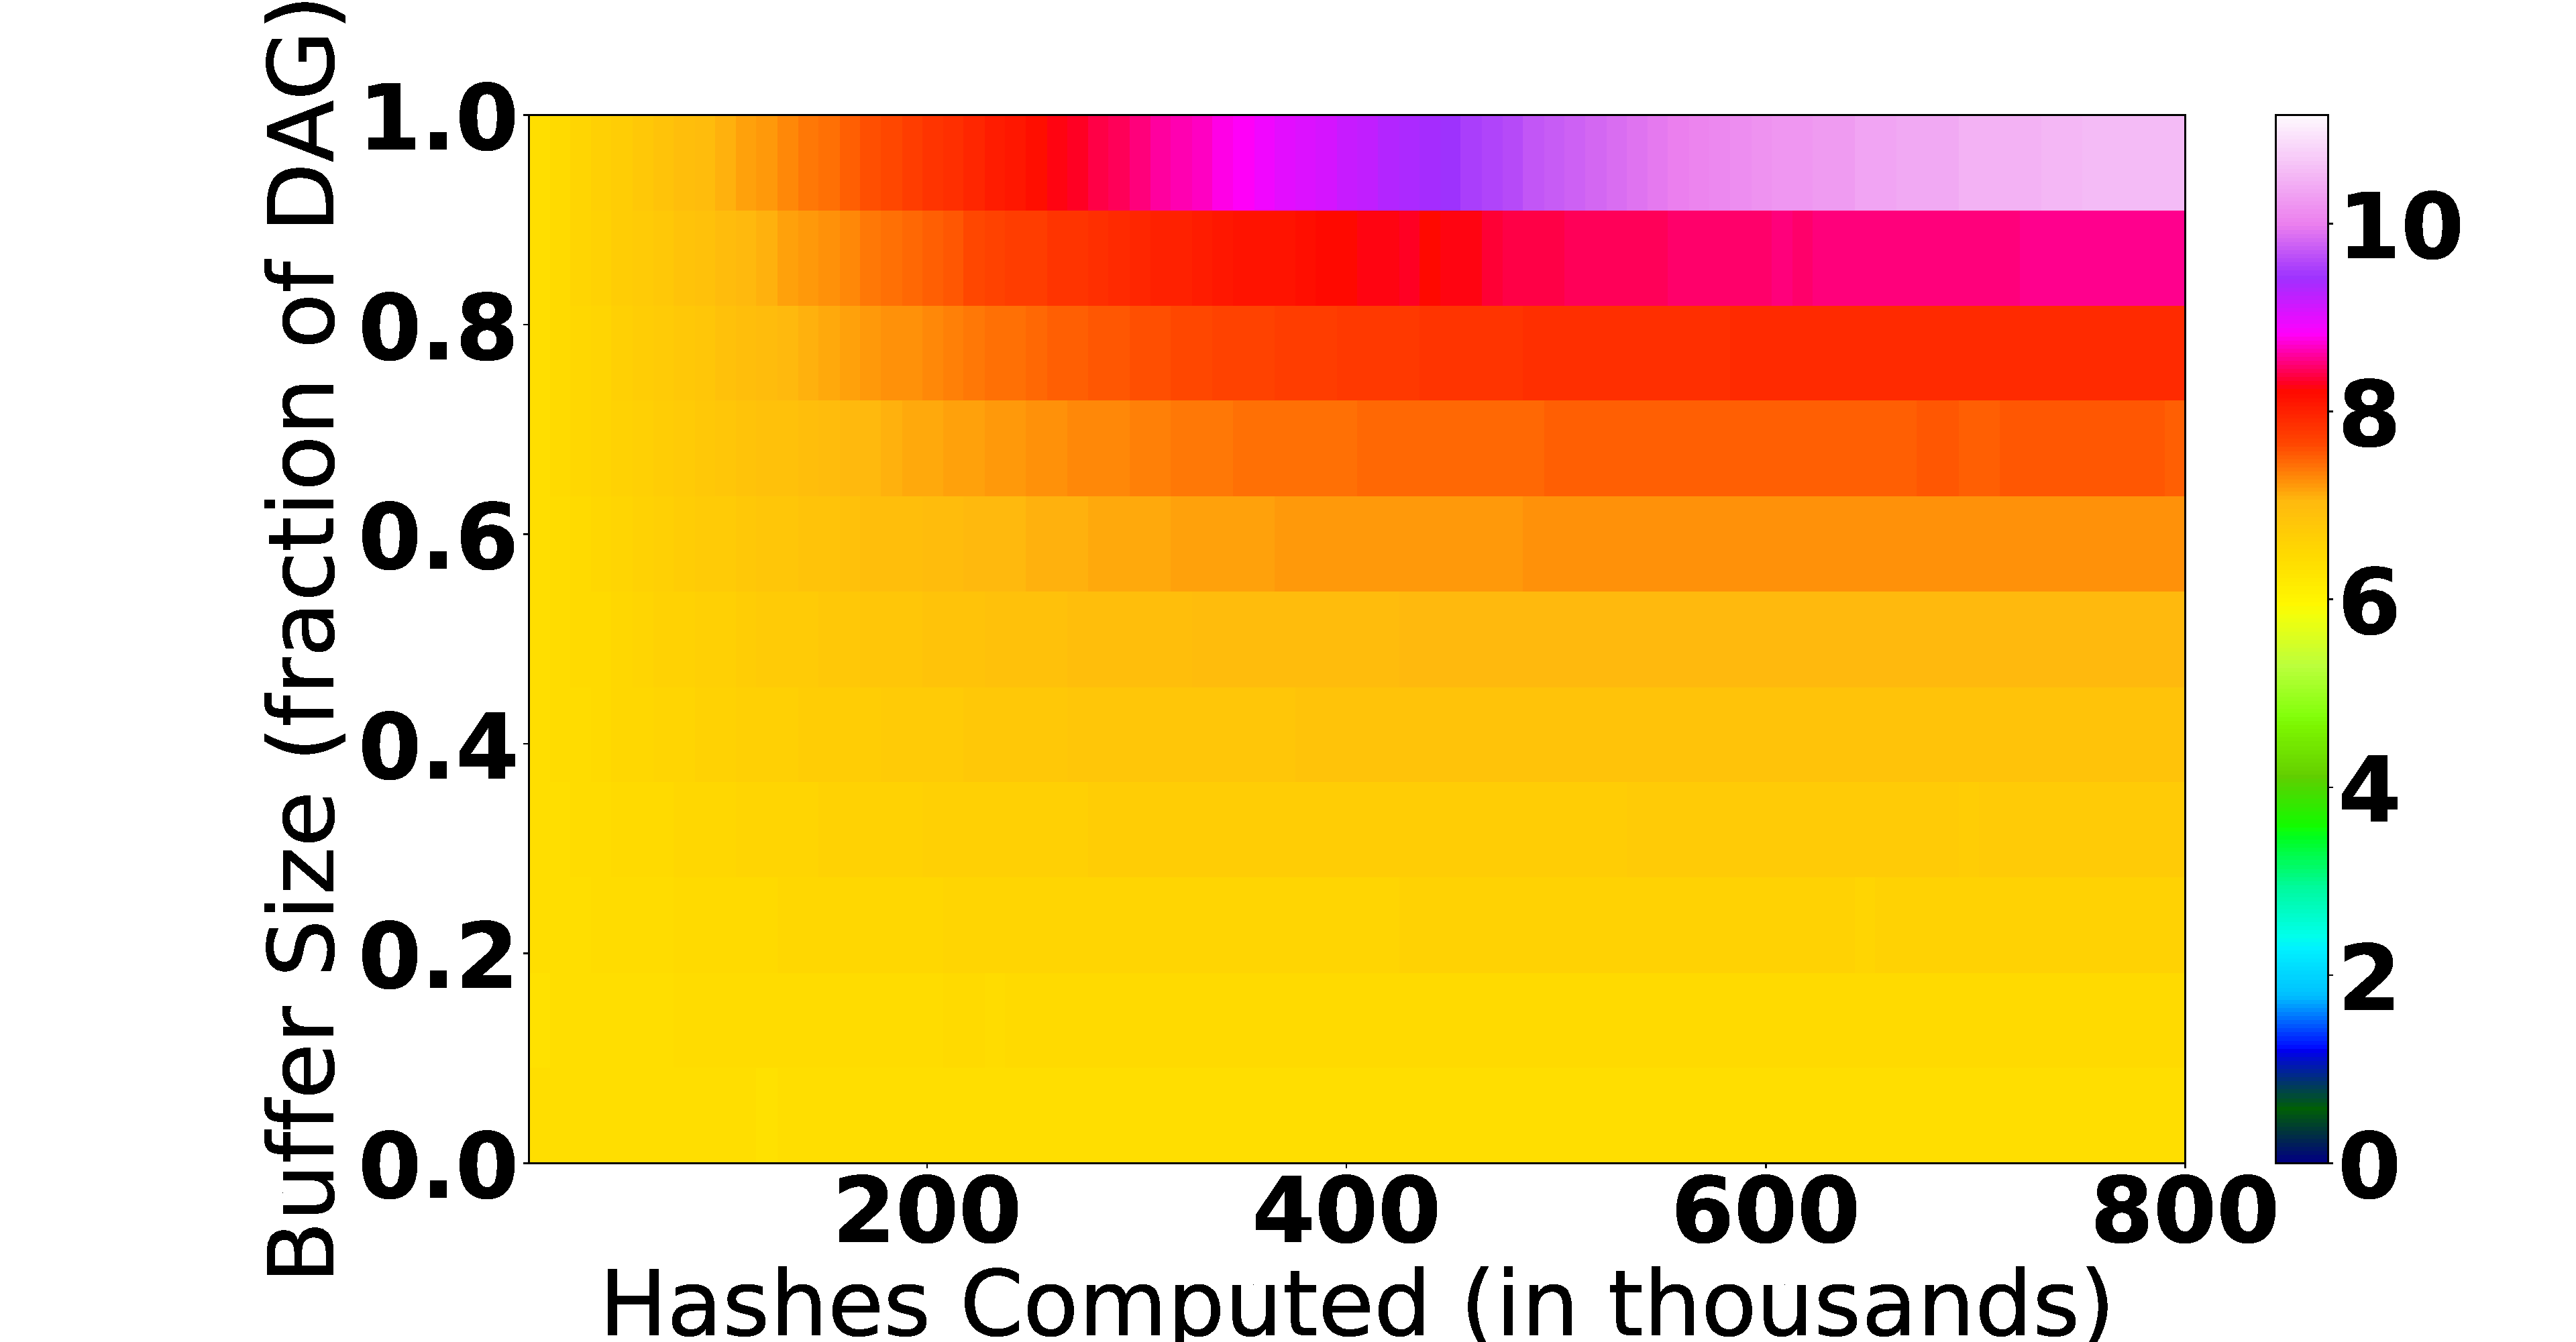
\includegraphics[width=\linewidth]{WebAssembly_Miner_Hash_Rate_HM.pdf}
% \endminipage\hfill
% \minipage{\textwidth}
%   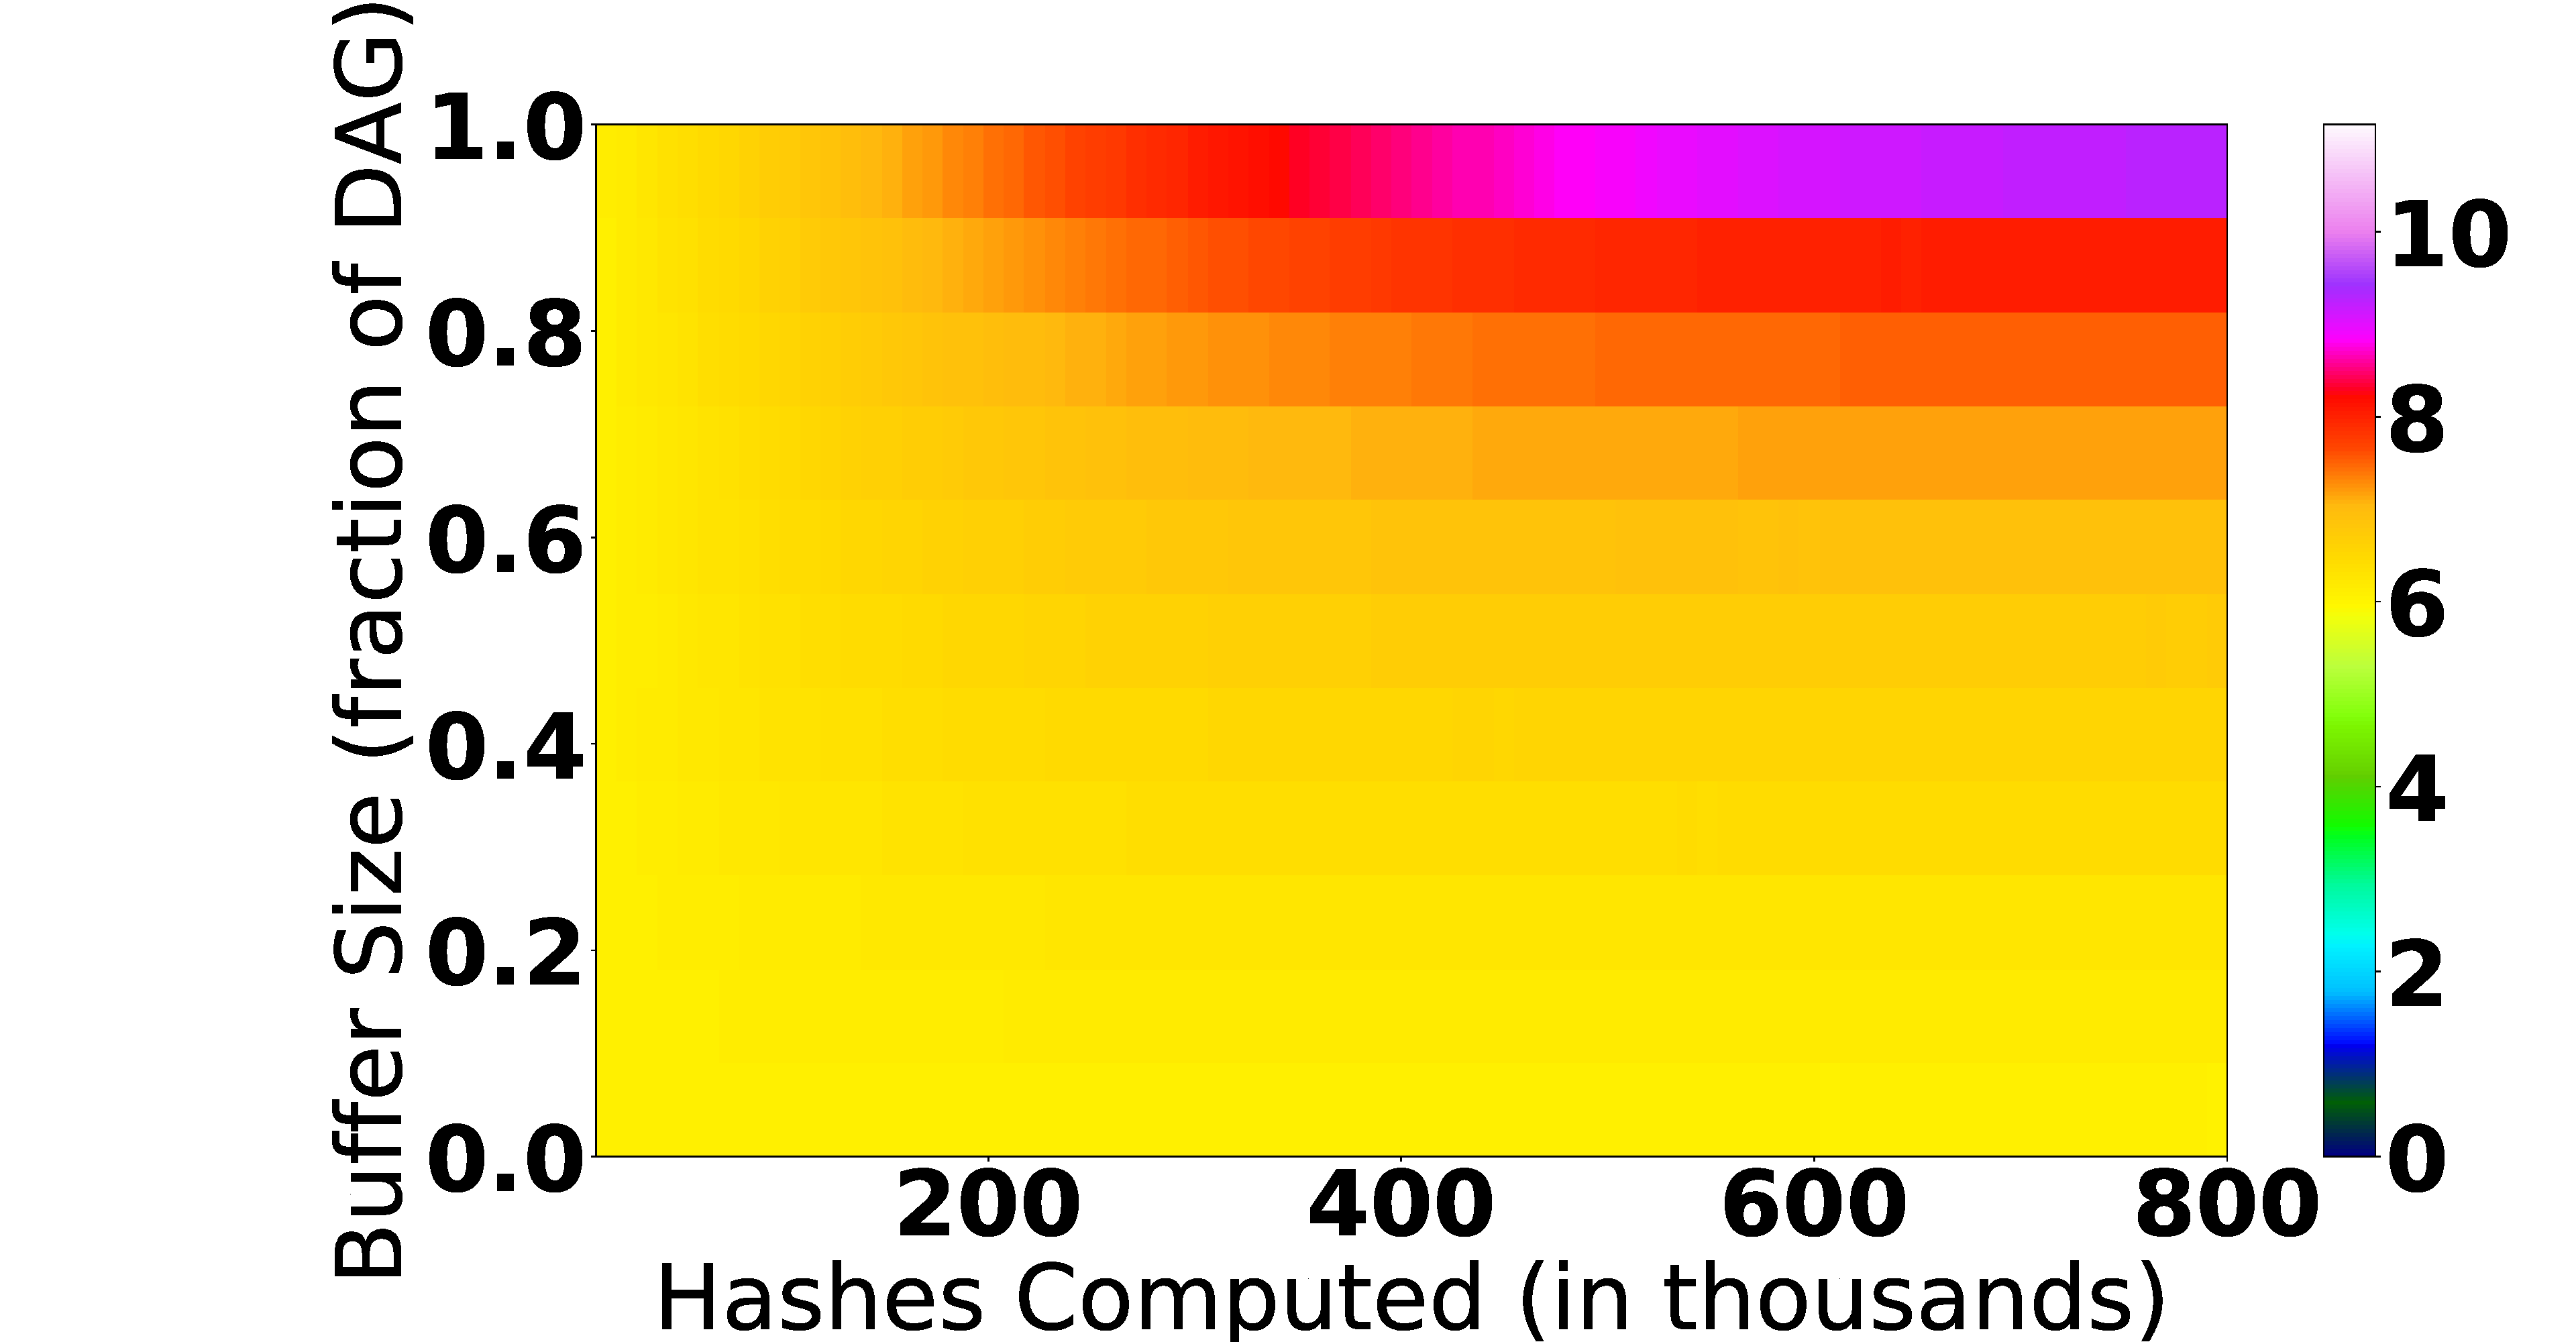
\includegraphics[width=\linewidth]{JavaScript_Miner_Hash_Rate_HM.pdf}
% \endminipage
% \caption{Hash Rate as a function of number of Hashes computed and Buffer Size}\label{fig:hashRateHM}
% \end{figure}

It is interesting to see how, for a given number of hashes computed, the hash rate drastically spikes up when the size of the buffer changes from 90\% of the size of the DAG to 100\%. This change becomes more apparent as the number of hashes computed increases -- thereby suggesting that accessing DAG slices from the buffer is orders of magnitude faster than computing them, so much so that even a few computations bring down the hash rate drastically. 

One way to reach the steady state hashrate faster for a given sized buffer would be to start out with a partially filled out buffer instead of an empty one. The only way this could work is by sending over part of the DAG over the network to the client. However, as it turns out, this is not feasible since, for a DAG with 16777186 slices (1.074 GB) sending even 10\% of the DAG would be sending $\approx100MB$ of data. With the global average download speed for desktops and smartphones being around 5.34MBps and 2.77MBps respectively ~\cite{internetSpeed}, the web page load time would be in the order of 20 seconds to a minute -- which is too long to get a mere 10\% boost in the buffer storage. 

The jump in the hash rate for high buffer hit rates is also seen in figure ~\ref{fig:bufferRatevsHashRate} where we show the correlations between the buffer hit rates and the hash rates for all 3 miners. The general trend is the same for all 3 miners -- the hash rate spikes up as the hit rate surpasses 95\% (Note that the hit rate gets extremely close to 1 but never quite reaches there, since we only compute 800k hashes as opposed to the 4.5 million would be needed as per our theoretical analysis).

\begin{figure}[h]
\centering
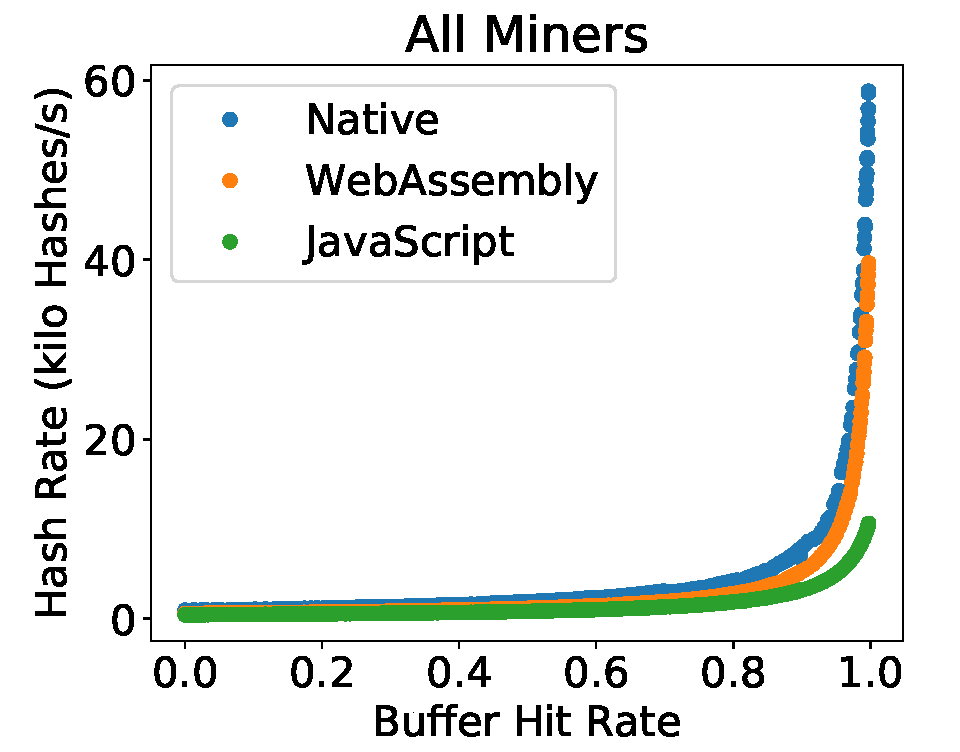
\includegraphics[width=250px,keepaspectratio]{All_Miners_Hash_Rate.pdf}
\caption{\label{fig:bufferRatevsHashRate} Buffer Hit Rate vs Hash Rate for all miners}
\end{figure}

Figure~\ref{fig:bufferRateHM} then shows a heat-map of how the DAG buffer hit-rate varies as a function of both the size of the buffer allocated to store the DAG and the number of hashes computed in the browser. 

\begin{figure}[H]
\centering
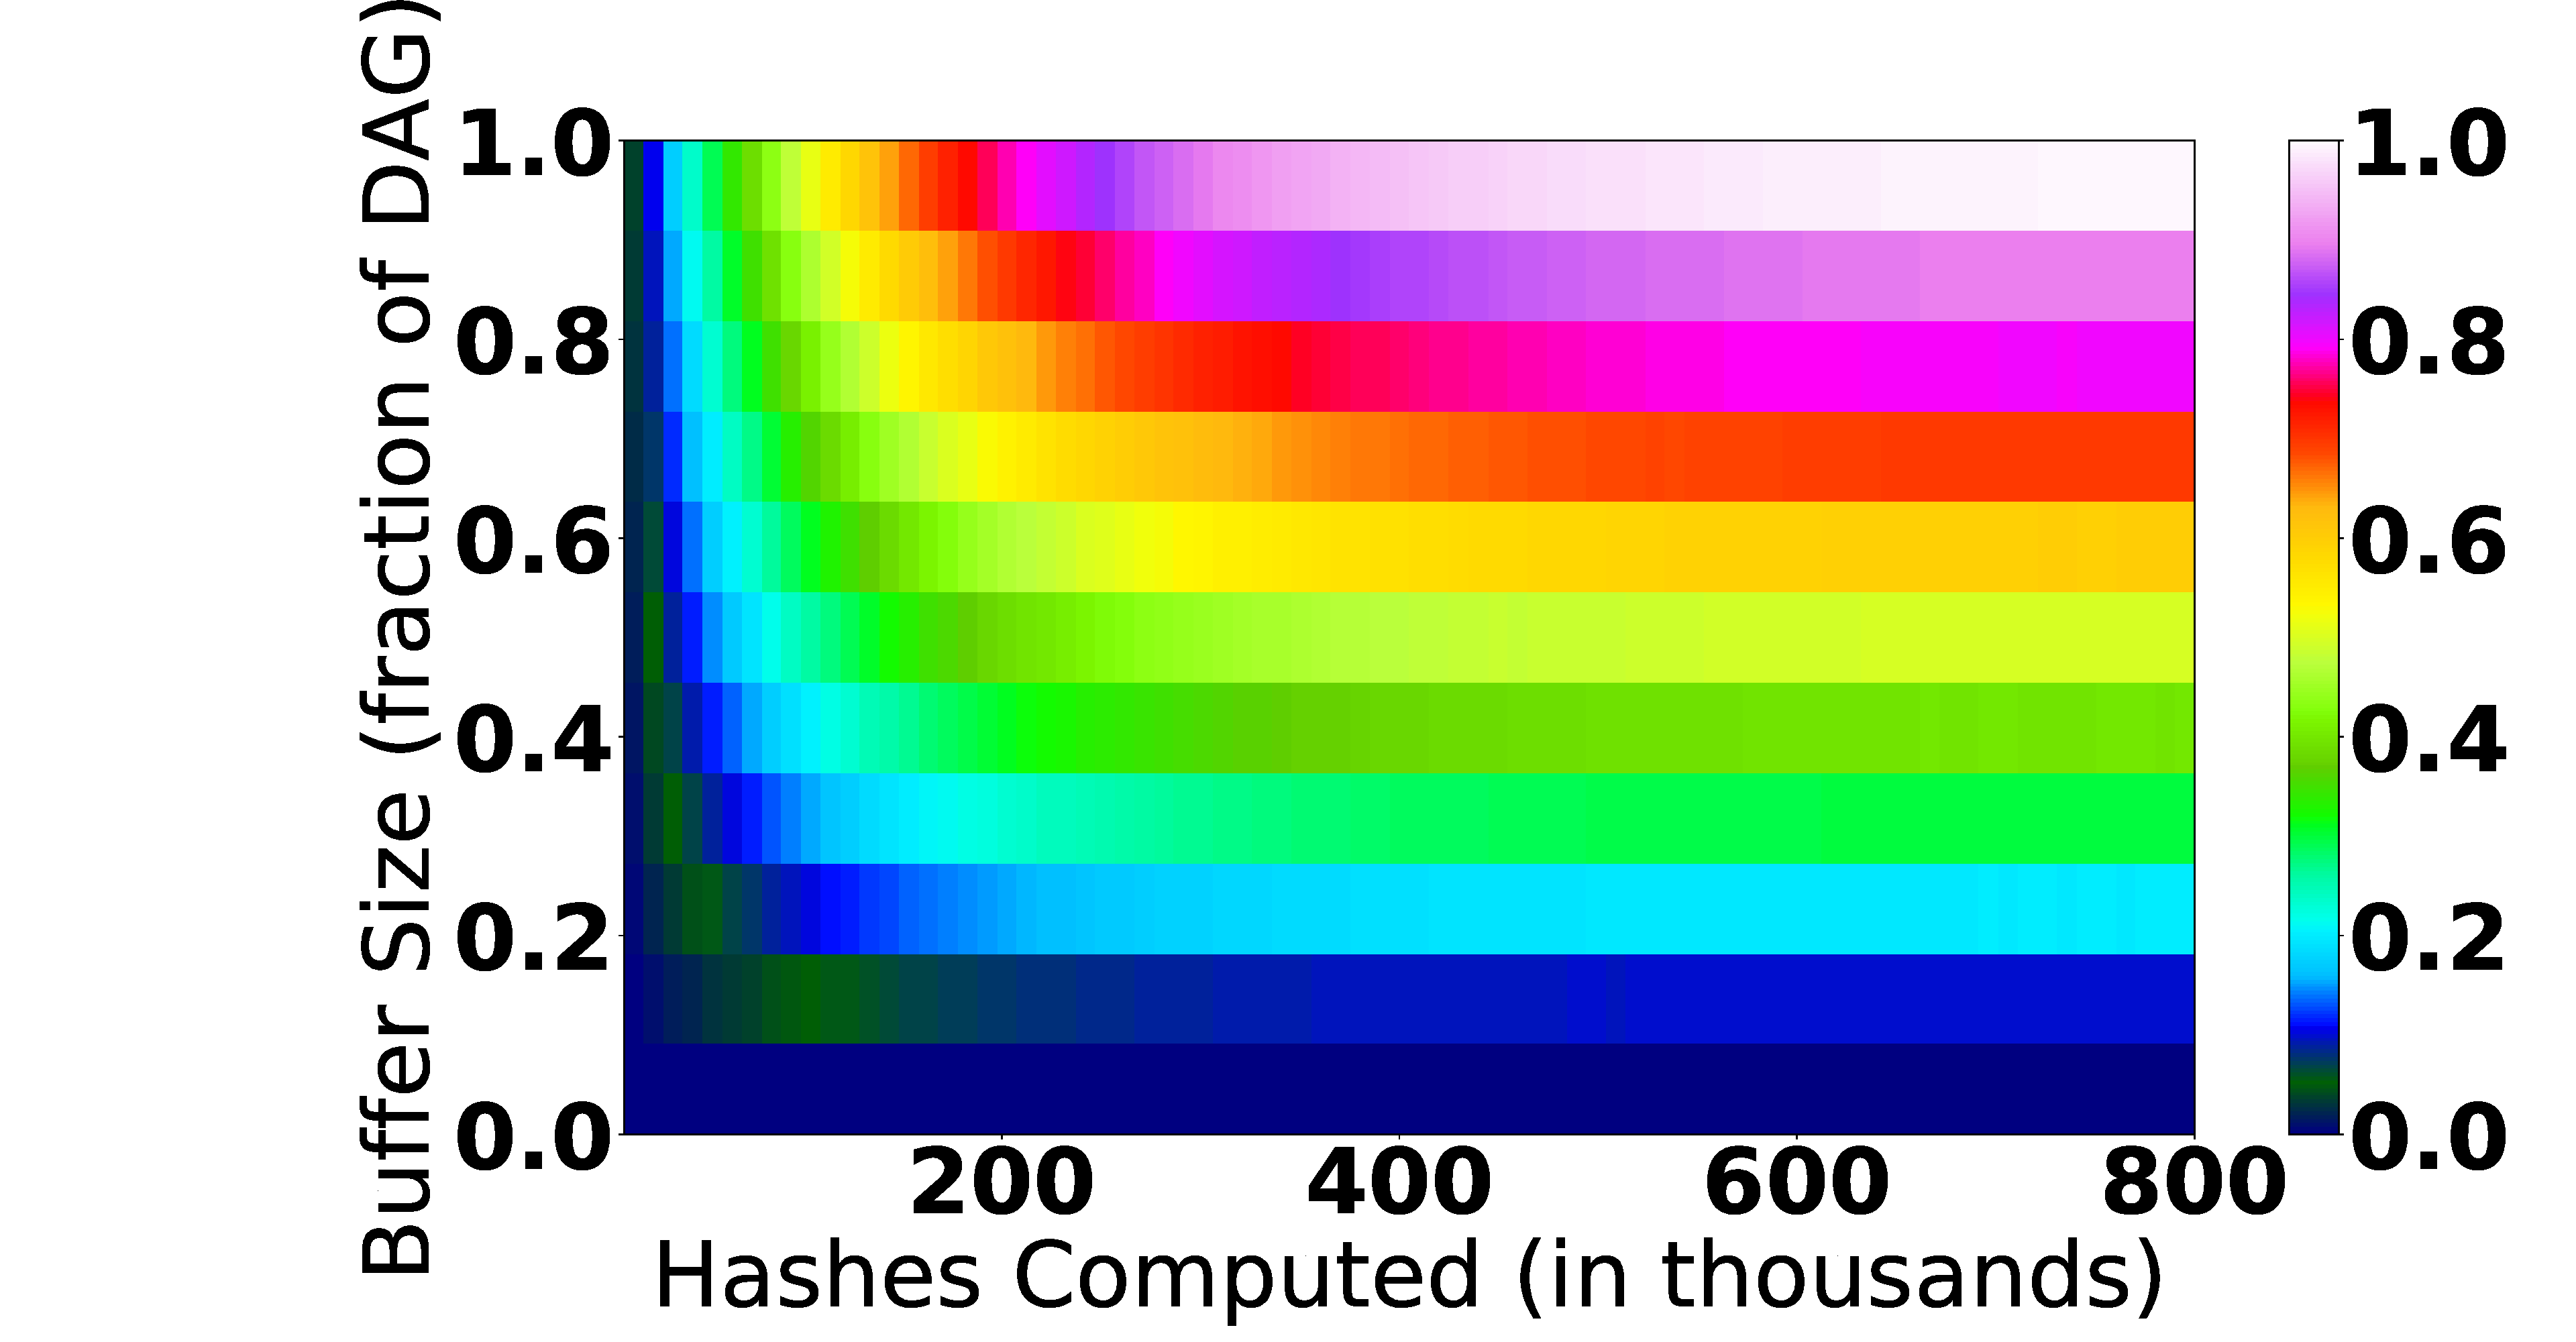
\includegraphics[width=250px,keepaspectratio]{All_Miners_Buffer_Hit_Rate.pdf}
\caption{\label{fig:bufferRateHM} Buffer Hit Rate}
\end{figure}

As expected, we see that the hit rate increases both with the size of the Buffer and with the number of hashes computed.

Table ~\ref{table:perf} shows us how the performance of each of the miners compare. Interestingly, the most conspicuous aspect is the fact that the performance variation between different implementations is not uniform across the buffer hit rate and the size of the buffer. We also see that for obvious reasons, the native miner outperforms both the ~\verb|JavaScript| and the ~\verb|WebAssembly| miner. However, we see that the ~\verb|WebAssembly| miner is at most 40.5\% slower than the native miner -- which is not very far off considering the overhead of running programs within browsers. The ~\verb|JavaScript| miner, on the other hand, is ~\textbf{at least} 47.2\% slower (and at most 82.0\% slower).

\begin{table}[t]
\caption{Performance Difference accross different Implementations}\label{table:perf}
\vspace{-2ex}
\begin{center}
\begin{tabular}{ c  c  c  c}

&\makecell{\textbf{WASM/JS}} & \makecell{\textbf{Native/JS}} & \makecell{\textbf{Native/WASM}}\\
\cline{2\ -2} \cline{3\ -3} \cline{4\ -4}
\makecell{\% Diff in smallest hash rate} & 35.9\% &  55.0\% & 38.9\% \\
\makecell{\% Diff in peak hash rate} & 73.2\% &  81.3\% & 30.2\% \\
\makecell{Min perf \% diff} &  24.4\% &  47.2\% & 23.9\% \\
\makecell{Max perf \% diff}  &  73.3\% &  82.0\% & 40.5\%\\ 
\makecell{Avg. Hash Rate \% diff \\
(averaged over all buffer sizes \\and cache hit rates)}&  30.6\% &  55.6\% & 35.9\%\\
\end{tabular}
\end{center}
\vspace{-3ex}
\end{table}



% \trishita{Got rid of figs 8 9 and 10 since we don't have much room}
% In Figures~\ref{fig:NativeWebAsm},~\ref{fig:WebAsmJS} and~\ref{fig:NativeJS} we show the percentage difference of the hashrates between the native miner and the browser miner implementations. We also compare the performance of the ~\verb|JavaScript| and ~\verb|WebAssembly|  miners.

% \begin{figure}[h]
% \centering
% \includegraphics[width=250px,keepaspectratio]{Native_Miner_vs_WebAssembly_miner_Hash_Rate_Percent_Improvement.pdf}
% \caption{\label{fig:NativeWebAsm} Native miner vs. WebAssembly miner Hash Rate Percent Improvement}
% \end{figure}

% \begin{figure}[h]
% \centering
% \includegraphics[width=250px,keepaspectratio]{WebAssembly_Miner_vs_JavaScript_miner_Hash_Rate_Percent_Improvement.pdf}
% \caption{\label{fig:WebAsmJS} WebAssembly miner vs. JavaScript miner Hash Rate Percent Improvement}
% \end{figure}

% \begin{figure}[h]
% \centering
% \includegraphics[width=250px,keepaspectratio]{Native_Miner_vs_JavaScript_miner_Hash_Rate_Percent_Improvement.pdf}
% \caption{\label{fig:NativeJS} Native miner vs. JavaScript miner Hash Rate Percent Improvement}
% \end{figure}


% \begin{figure}[!htb]
% \minipage{0.32\textwidth}
%   \includegraphics[width=\linewidth]{WebAssembly_Miner_vs_JavaScript_miner_Hash_Rate_Percent_Improvement.pdf}
% \endminipage\hfill
% \minipage{0.32\textwidth}
%   \includegraphics[width=\linewidth]{Native_Miner_vs_WebAssembly_miner_Hash_Rate_Percent_Improvement.pdf}
% \endminipage\hfill
% \minipage{0.32\textwidth}
%   \includegraphics[width=\linewidth]{Native_Miner_vs_JavaScript_miner_Hash_Rate_Percent_Improvement.pdf}
% \endminipage
% \caption{Percentage difference in Hash Rates for different miner implementations}\label{fig:PerfChangeHM}
% \end{figure}

Finally, we tabulate the most important results from our analysis in table ~\ref{table:results}
\trishita{To Do: Fill in other, meaningful, metrics -- any suggestions?}

\begin{table}[t]
\caption{Main Results}\label{table:results}
\vspace{-2ex}
\begin{center}
\begin{tabular}{ c  c  c  c}

&\makecell{\textbf{Native}} & \makecell{\textbf{JavaScript}} & \makecell{\textbf{WebAssembly}}\\
\cline{2\ -2} \cline{3\ -3} \cline{4\ -4}
\makecell{Median Hash Rate \\
(for a buffer the size of the DAG)} & 15278H/s &  5290H/s & 10504H/s \\
Peak Hash Rate &  56800H/s &  10626H/s & 39651H/s \\
\makecell{Maximum Time to reach steady state \\ hash rate (buffer as large as DAG)}  &  X s &  X s & X s\\ 
\makecell{Avg. Hash Rate \% diff with Native Miner \\
(averaged over all buffer sizes)}&  NA &  55.6\% & 35.9\%\\
\end{tabular}
\end{center}
\vspace{-3ex}
\end{table}


% Note that this is the computational power of one machine and in reality, there would be hundreds or thousands of machines mining simultaneously, which will be analyzed in the next section. In comparison to Monero or Bitcoin browser miners who mine on an average of about 30-60H/s, our hashrate is significantly better than those.

\section{Conclusion}
We have successfully created a proof of concept distributed, web-based Ethereum miner that can be used towards monetizing electronic content, web-authentication rate limiting, private test networks, user tracking for advertisers, etc. Our implementation is standalone, and hence can simply be embedded within a website without having the client install any external dependencies. We get the best steady state hash rates for our \verb|JavaScript| and \verb|WebAssembly| implementations (10.6k and 39.6k respectively) when the cache hit rates approach 1, (which takes approx 800k Hashes). 

% Furthermore, we provide an API that can be used by any implementation of Ethereum (\verb|geth| or Ethereum's implementation in \verb|C++|). We believe this can be a be especially viable in a private testnet, within a company for example, and with further research has the potential to make a real impact.

\section{Future Work}
While we were able to create a browser based miner for Ethereum, there is still work to be done. As was shown, our current implementation is far slower than the traditional methods for mining. One way we can look to speed this process up is to tap into the client machine's GPU. There is a \verb|JavaScript| library called WebCL that binds to the OpenCL library which allows the \verb|JavaScript| to speak directly to the GPU for better parallel performance. Knowing that Ethereum was created for GPU mining and based on our results, it should provide a substantial improvement. 
% In addition, because of the memory hard requirements of the Ethereum protocol we should also see a better performance if we can somehow get the DAG to be directly accessible to the client instead of having to send slices over the network to all the clients. Therefore, we want to look into the use of \verb|remoteStorage| ~\cite{remote}, which allows the user to have complete control over the data. By moving the data closer to the computation we are hoping to cut the added time caused by the network.
Ethereum is also currently working on Casper, their Proof-of-Stake algorithm, which has already been deployed to private testnets for testing. Working with that and the fact that Casper is open-source, it would be possible to create a theoretical Proof-of-Stake distributed browser miner implementation in preparation for the fork. However, seeing as though Proof-of-Stake would virtually eliminate the necessity of massive amounts of processing power, users would most likely have to provide ``stakes" in order for such an implementation to be possible ~\cite{PoSproof}. Further research will be necessary to determine whether browser mining for Casper is viable or not, as the final form of Casper is still hazy and exactly how much ``stake'' is required to mine is uncertain.


% conference papers do not normally have an appendix


% % use section* for acknowledgement
\section*{Acknowledgment}
The authors would like to thank Dennis Your for his contributions to this work.

\begin{thebibliography}{1}
\bibitem{Adblock} Gundlach, Micheal. AdBlock browser extension. AdBlock. Software, 2009.

\bibitem{ethash}Matthew Wampler, et al. Ethash. Computer software. GitHub. Vers. 23.1. GitHub, 11 Jan. 2015. Web. 24 Feb. 2018. <https://github.com/ethereum/ethash>. 

\bibitem{BraveBrowser} Eich, Brendan and Brian Bondy. Brave Browser. Brave Software. Software, 2015.

\bibitem{decliningRevenue} Hern, Alex. “Adblock Plus: the Tiny Plugin Threatening the Internet's Business Model.” The Guardian, Guardian News and Media, 14 Oct. 2013, www.theguardian.com/technology/2013/oct/14/the-tiny-german-company-threatening-the-internets-business-model.

\bibitem{dagger-hashimoto} Buterin, Vitalik, et al. “Ethereum/Wiki.” GitHub, GitHub, 9 Feb. 2014, github.com/ethereum/wiki/blob/master/Dagger-Hashimoto.md. 

\bibitem{noSubscriptions} Rosenwald, Micheal. “Digital News Consumers Unlikely to Pay for Content and Increasingly Block Ads.” Columbia Journalism Review, Columbia Journalism Review, 15 June 2015, www.cjr.org/analysis/reuters\_digital\_news\_report.php.

\bibitem{payPerClick} Fessenden, Therese. “Nielsen Norman Group.” The Most Hated Online Advertising Techniques, Nielsen Norman Group, 4 June 2017, www.nngroup.com/articles/most-hated-advertising-techniques/.

\bibitem{celebEndorse} Awad, Amal. “A Study in Scarlett: The Ethics of Celebrity Endorsement.” – Opinion – ABC Religion \&Amp; Ethics (Australian Broadcasting Corporation), Amal Awad ABC Religion and Ethics, 30 Jan. 2014, www.abc.net.au/religion/articles/2014/01/31/3935443.htm.

% \bibitem{Boldrin} Boldrin, F., et al. “Distributed Computing Through Web Browser.” Distributed Computing Through Web Browser - IEEE Conference Publication, University of Ferrara, ieeexplore.ieee.org/document/4350073/.

\bibitem{scheduling}
Ramamritham, Krithi, and John A. Stankovic. "Dynamic task scheduling in hard real-time distributed systems." IEEE software 1.3 (1984): 65.

\bibitem{parallel}
Shirazi, Behrooz A., Krishna M. Kavi, and Ali R. Hurson. Scheduling and load balancing in parallel and distributed systems. IEEE Computer Society Press, 1995.

\bibitem{orca}
Bal, Henri E., M. Frans Kaashoek, and Andrew S. Tanenbaum. "Orca: A language for parallel programming of distributed systems." IEEE transactions on software engineering 18.3 (1992): 190-205.

\bibitem{WebFlow}
Bhatia, Dimple; Burzevski, Vanco; Camuseva, Maja; and Fox, Geoffrey C., "WebFlow - A Visual Programming Paradigm for Web/Java Based Coarse Grain Distributed Computing" (1997).
Northeast Parallel Architecture Center.

\bibitem{Cushing} Cushing, Reginald, et al. “Distributed Computing on an Ensemble of Browsers.” IEEE Internet Computing, IEEE, 1 Sept. 2013, www.computer.org/csdl/mags/ic/2013/05/mic2013050054.html.

\bibitem{randmemohash} Lerner, Sergio Demian. "STRICT MEMORY HARD HASHING FUNCTIONS (PRELIMINARY V0. 3, 01-19-14)."

\bibitem{coinhive}
The Coinhive Team. Coinhive browser extension. Coinhive. Software, 2017.

\bibitem{pow}
Laurie, Ben, and Richard Clayton. "Proof-of-work proves not to work; version 0.2." Workshop on Economics and Information, Security. 2004.

\bibitem{casper}
Hertig, Alyssa. “Ethereum's Big Switch: The New Roadmap to Proof-of-Stake.” CoinDesk, CoinDesk, 16 May 2017, www.coindesk.com/ethereums-big-switch-the-new-roadmap-to-proof-of-stake/. 

\bibitem{pos}
Dmitry Buterin, et al. “Proof of Work vs Proof of Stake: Basic Mining Guide.” Blockgeeks, Blockgeeks, 24 July 2017, blockgeeks.com/guides/proof-of-work-vs-proof-of-stake/. 

\bibitem{arc}
The ArcticCoin Team. ArcticCoin crypto-currency. ArcticCoin. Software, 2015.

\bibitem{Monero} “Monero - Secure, Private, Untraceable.” Getmonero.org, The Monero Project, getmonero.org/.

\bibitem{Duda} Duda, Jerzy, and Wojciech Dłubacz. “Distributed Evolutionary Computing System Based on Web Browsers with Javascript.” ACM Digital Library, Springer-Verlag, dl.acm.org/citation.cfm?id=2451764.2451780.

\bibitem{traffic} The SimilarWeb Team. SimilarWeb LTD 2017. (https://www.similarweb.com/)

\bibitem{coinwarz}Coinwarz Ethereum Mining Calculator and Profit Calculator. Coinwarz 2017. (https://www.coinwarz.com/calculators/ethereum-mining-calculator)

\bibitem{PoSproof}Dale, Oliver. "Beginner's Guide to Ethereum Casper Hardfork: What You Need to Know". Blocknomi, 7 November 2017. (https://blockonomi.com/ethereum-casper/)

\bibitem{Ethmining}
Wood, Gavin. "Ethereum: A secure decentralised generalised transaction ledger." Ethereum Project Yellow Paper 151 (2014): 1-32.

\bibitem{geth}Péter Szilágyi, et al. Geth. Computer software. GitHub. Vers. 1.8.1. GitHub, 22 Dec. 2013. Web. 24 Feb. 2018. <https://github.com/ethereum/go-ethereum>. 

\bibitem{etherscan}Etherscan The Ethereum Block Explorer. Etherscan 2017. (https://etherscan.io/charts)

\bibitem{remote} remoteStorage: An open protocol for per-user storage on the Web. (https://remotestorage.io/)

\bibitem{webAssembly}  W3C Team. WebAssembly. Program documentation. WebAssembly. Vers. 1.0. WebAssembly, 17 Mar. 2017. Web. 28 Mar. 2018. <http://webassembly.org>. 

\bibitem{wasmPerf} Zlatkov, Alexander. "How JavaScript Works: A Comparison with WebAssembly." SessionStack Blog. SessionStack Blog, 21 Nov. 2017. Web. 28 Mar. 2018. <https://blog.sessionstack.com/how-javascript-works-a-comparison-with-webassembly-why-in-certain-cases-its-better-to-use-it-d80945172d79>. 

\bibitem{emscripten} Emscripten Community. Emscripten. Emscripten. Vers. 1.37.36. Emscripten, 11 Nov. 2012. Web. 28 Mar. 2018. <http://kripken.github.io/emscripten\-site/docs/getting\_started/Tutorial.html>. 

\bibitem{internetSpeed} Ookla. “Speedtest Global Index – Monthly Comparisons of Internet Speeds from around the World.” Speedtest Global Index, Ookla, 25 Mar. 2018, www.speedtest.net/global-index.
\bibitem{hydra}  Fogerlie, Garrett, director. Brute Force Website Login Attack Using Hydra - Hack Websites - Cyber Security. Brute Force Website Login Attack Using Hydra - Hack Websites - Cyber Security, YouTube, 24 Sept. 2013, www.youtube.com/watch?v=ZVngjGp-oZo. 

\bibitem{burpsuite} Mahmood, Osama. “Brute Force Website Login Page Using Burpsuite –.” SecurityTraning, SecurityTraning, 5 Feb. 2018, securitytraning.com/brute-force-website-login-page-using-burpsuite/. 

\bibitem{webLogsManipulation} Fox\-Brewster, Thomas. ``'Biggest Ad Fraud Ever': Hackers Make \$5M A Day By Faking 300M Video Views.'' Forbes, Forbes Magazine, 20 Dec. 2016, www.forbes.com/sites/thomasbrewster/2016/12/20/methbot\-biggest\-ad\-fraud\-busted/\#73f089a94899/ 

\bibitem{couponCollector} Neal, Peter. ``The Generalised Coupon Collector Problem.'' Journal of Applied Probability, vol. 45, no. 3, 2008, pp. 621\-629., doi:10.1239/jap/1222441818.
\bibitem{harmonicNumber} Guo, Bai-Ni \& Qi, Feng. (2011). Sharp bounds for harmonic numbers. Applied Mathematics and Computation. 218. 991-. 10.1016/j.amc.2011.01.089.
\end{thebibliography}

\addtolength{\textheight}{-7cm}
\balance


% that's all folks
\end{document}